%definira klasu dokumenta 

\documentclass[12pt]{report} 

%prostor izmedu naredbi \documentclass i \begin{document} se zove uvod. U njemu se nalaze naredbe koje se odnose na cijeli dokument

%osnovni LaTex ne može riješiti sve probleme, pa se koriste različiti paketi koji olakšavaju izradu željenog dokumenta
\usepackage[croatian]{babel} 
\usepackage{amssymb}
\usepackage{amsmath}
\usepackage{txfonts}
\usepackage{mathdots}
\usepackage{titlesec}
\usepackage{array}
\usepackage{lastpage}
\usepackage{etoolbox}
\usepackage{longtable, tabu}
\usepackage{color, colortbl}
\usepackage{adjustbox}
\usepackage{geometry}
\usepackage[classicReIm]{kpfonts}
\usepackage{hyperref}
\usepackage{fancyhdr}

\usepackage{float}
\usepackage{setspace}
\restylefloat{table}


\patchcmd{\chapter}{\thispagestyle{plain}}{\thispagestyle{fancy}}{}{} %redefiniranje stila stranice u paketu fancyhdr

%oblik naslova poglavlja
\titleformat{\chapter}{\normalfont\huge\bfseries}{\thechapter.}{20pt}{\Huge}
\titlespacing{\chapter}{0pt}{0pt}{40pt}


\linespread{1.3} %razmak između redaka

\geometry{a4paper, left=1in, top=1in,}  %oblik stranice

\hypersetup{ colorlinks, citecolor=black, filecolor=black, linkcolor=black,	urlcolor=black }   %izgled poveznice


%prored smanjen između redaka u nabrajanjima i popisima
\newenvironment{packed_enum}{
	\begin{enumerate}
		\setlength{\itemsep}{0pt}
		\setlength{\parskip}{0pt}
		\setlength{\parsep}{0pt}
	}{\end{enumerate}}

\newenvironment{packed_item}{
	\begin{itemize}
		\setlength{\itemsep}{0pt}
		\setlength{\parskip}{0pt}
		\setlength{\parsep}{0pt}
	}{\end{itemize}}


%boja za privatni i udaljeni kljuc u tablicama
\definecolor{LightBlue}{rgb}{0.9,0.9,1}
\definecolor{LightGreen}{rgb}{0.9,1,0.9}


%podesavanje zaglavlja i podnožja

\pagestyle{fancy}
\lhead{Programsko inženjerstvo}
\rhead{Znanstvena konferencija}
\lfoot{Grupa1}
\cfoot{stranica \thepage/\pageref{LastPage}}
\rfoot{\today}
\renewcommand{\headrulewidth}{0.2pt}
\renewcommand{\footrulewidth}{0.2pt}


\begin{document} 
	
	
	
	\begin{titlepage}
		\begin{center}
			\vspace*{\stretch{1.0}} %u kombinaciji s ostalim \vspace naredbama definira razmak između redaka teksta
			\LARGE Programsko inženjerstvo\\
			\large Ak. god. 2020./2021.\\
			
			\vspace*{\stretch{3.0}}
			
			\huge Znanstvena konferencija\\
			\Large Dokumentacija, Rev. \textit{2}\\
			
			\vspace*{\stretch{12.0}}
			\normalsize
			Grupa: \textit{Grupa1}\\
			Voditelj: \textit{Marko Andreis}\\
			
			
			\vspace*{\stretch{1.0}}
			Datum predaje: \textit{14. siječnja 2020.}\\
	
			\vspace*{\stretch{4.0}}
			
			Nastavnik: \textit{Miljenko Krhen}\\
		
		\end{center}

	
	\end{titlepage}

	
	\tableofcontents

	\chapter{Dnevnik promjena dokumentacije}		
		
		\begin{longtabu} to \textwidth {|X[2, l]|X[13, l]|X[3, l]|X[3, l]|}
			\hline \multicolumn{1}{|l|}{\textbf{Rev.}}	& \multicolumn{1}{l|}{\textbf{Opis promjene/dodatka}} & \multicolumn{1}{|l|}{\textbf{Autori}} & \multicolumn{1}{l|}{\textbf{Datum}} \\[3pt] \hline
			\endfirsthead
			
			\hline \multicolumn{1}{|l|}{\textbf{Rev.}}	& \multicolumn{1}{l|}{\textbf{Opis promjene/dodatka}} & \multicolumn{1}{|l|}{\textbf{Autori}} & \multicolumn{1}{l|}{\textbf{Datum}} \\[3pt] \hline
			\endhead
			
			\hline 
			\endlastfoot
			
			0.1 & Dodana struktura za početak rada na dokumentaciji & Andreis & 21.10.2020. 		\\[3pt] \hline 
			0.2	& Započet rad na opisu projekta & Bašić & 24.10.2020. 	\\[3pt] \hline
			0.2.1	& Dovršen opis projektnog zadatka & Andreis & 27.10.2020. 	\\[3pt] \hline
			0.3 & Dodani funkcionalni zahtjevi i nefunkcionalni zahtjevi & Majstorović & 28.10.2020. \\[3pt] \hline
			0.4.1 & Dodan prvi dio opisa obrazaca uporabe & Andreis & 29.10.2020. 		\\[3pt] \hline
			0.5 & Dodani svi opisi obrazaca uporabe & Bašić, Matić & 30.10.2020. 		\\[3pt] \hline
			0.5.1 & Prepravljen prvi dio obrazaca uporabe & Krešo, Pasković & 01.11.2020. 		\\[3pt] \hline
			0.5.2 & Prepravljen drugi dio obrazaca uporabe & Majstorović & 02.11.2020. 		\\[3pt] \hline
			0.5.3 & Ispravak obrazaca uporabe & Andričević & 04.11.2020. 		\\[3pt] \hline  
			0.5.4 & Ispravak obrazaca uporabe & Andreis & 04.11.2020. 		\\[3pt] \hline
			0.6 & Dodan \textit{Use Case} dijagram, dovršeni funkcionalni i nefunkcionalni zahtjevi & Matić, Pasković & 05.11.2020. \\[3pt] \hline 
			0.6.1 & Dodani novi obrasci uporabe & Majstorović & 05.11.2020. 		\\[3pt] \hline
			0.6.2 & Izmjena dijagrama obrazaca uporabe & Andričević & 06.11.2020. 		\\[3pt] \hline
			0.6.3 & Dodan novi obrazac uporabe, izmjena dijagrama & Bašić, Krešo & 06.11.2020. 		\\[3pt] \hline
			0.7 & Dodani sekvencijski dijagrami & Andreis, Matić & 07.11.2020. 		\\[3pt] \hline
			0.7.1 & Popravljeni sekvencijski dijagrami i dijagrami obrazaca uporabe & Pasković & 07.11.2020. 		\\[3pt] \hline
			0.8 & Arhitektura i dizajn sustava & Bašić, Matić, Andreis & 08.11.2020. 		\\[3pt] \hline
			0.8.1 & Zaključak i budući rad, dodatak A, B i C & Krešo, Pasković & 09.11.2020. 		\\[3pt] \hline
			0.8.2. & Dijagram objekata & Majstorović & 09.11.2020. 		\\[3pt] \hline
			0.8.3 & Pojmovnik & Andričević & 10.11.2020. 		\\[3pt] \hline
			0.9.1 & Popravljena baza podataka & Bašić, Krešo & 11.11.2020. 		\\[3pt] \hline
			0.9.2 & Dijagram razreda i dijagram objekata & Matić, Pasković & 11.11.2020. 		\\[3pt] \hline
			0.9.2 & Opisi razreda i dodatak D & Andričević & 12.11.2020. 		\\[3pt] \hline
			\textbf{1.0} & Korigiranje teskta i provjera dokumentacije & Andreis & 13.11.2020. 		\\[3pt] \hline
			1.1 & Dodan dijagram stanja & Andričević &  03.12.2020. 		\\[3pt] \hline
			1.1.1 & Popravljen dijagram stanja & Pasković & 05.12.2020. 		\\[3pt] \hline
			1.2 & Dodan dijagram aktivnosti & Matić & 09.12.2020. 		\\[3pt] \hline
			1.3 & Dodan dijagram komponenti & Matić & 11.12.2020. 		\\[3pt] \hline
			1.3.1 & Popravljen dijagram komponenti & Andričević & 13.12.2020. 		\\[3pt] \hline
			1.4 & Ispisane tehnologije i alati & Andreis, Majstorović & 18.12.2020. 		\\[3pt] \hline
			1.5. & Provedeno ispitivanje komponenti i sustava & Andreis, Krešo, Matić, Bašić & 20.12.2020. 		\\[3pt] \hline
			1.5.1 & Dodan dijagram razmještaja & Pasković & 21.12.2020. 		\\[3pt] \hline
			1.6 & Napisane upute za puštanje u pogon & Majstorović, Andreis & 04.01.2021. 		\\[3pt] \hline
			1.6.1 & Nadopunjene upute za puštanje u pogon & Andričević, Matić & 06.01.2021. 		\\[3pt] \hline
			1.6.2 & Ispravljenje greške u uputama za puštanje u pogon & Andreis & 08.01.2021. 		\\[3pt] \hline
			1.7 & Napisan zaključak & Pasković & 09.01.2021. 		\\[3pt] \hline
			1.8 & Nadopunjen popis literature & Majstorović & 09.01.2021. 		\\[3pt] \hline
			1.9 & Nadopunjeni dnevnik sastajanja, dnevnik promjena dokumentacije i tablica aktivnosti & Pasković, Andreis, Bašić & 12.01.2021. 		\\[3pt] \hline
			\textbf{2.0} & Korigiranje teksta i provjera dokumentacije & Andreis & 14.01.2021 		\\[3pt] \hline
								
		\end{longtabu}
	
	
	\chapter{Opis projektnog zadatka}
		
		Cilj ovog projekta je implementacija učinkovitog informacijskog sustava naziva \textit{"Sci-Con"} za organiziranje, upravljanje i sudjelovanje na znanstvenim konferencijama. Sustav je namijenjen organizatorima konferencija koji će korištenjem sustava biti u mogućnosti stvarati nove konferencije na koje će se budući sudionici znanstvenih konferencija moći prijavljivati i svojim sudjelovanjem dobiti priliku za prezentiranje vlastitih znanstvenih radova. Dodatno, sustav omogućava korisnicima s ovlastima recenzenta pregledavanje i ocjenjivanje radova svih korisnika kojima je ranije potvrđena prijava na konferenciju kao i slanje povratne informacije vezane za opći dojam o pregledanom znanstvenom radu. Informacijski sustav opisan u uvodnom dijelu bit će dostupan na web stranici organizatora konferencije.\\
		     
		    
		\textit Sustav mora biti u mogućnosti pružiti potporu za definiranje početnih postavki svake nove konferencije. Stvaranje nove konferencije inicira organizator konferencija upitom \underbar{administratoru} koji na zadanu inicijativu odgovara definiranjem novog upitnika za prijavu na konferenciju kojeg prilikom prijave ispunjavaju sudionici konferencije. Dodatno, prilikom postavljanja početnih postavki, administrator postavlja i organizatora konferencije. U svakom trenutku rada sustava, administrator ima mogućnost pregleda broja i imena trenutno prijavljenih korisnika i ukupnog broja korisnika registriranih u sustav. Također, sustav omogućava istovremeni rad administratora i neograničenog broja registriranih korisnika.\\
		
		\textit Svaki u sustav \underbar{neregistrirani korisnik} mora obaviti registraciju prije korištenja funkcionalnosti koje sustav pruža. Korisnik prilikom registracije obavezan je ispuniti obrazac koji uključuje sljedeće podatke: 
		
		\begin{packed_item}
			
			\item ime
			\item prezime
			\item naziv institucije ili poduzeća u kojem djeluje
			\item adresu boravka
			\begin{packed_item}
				\item ulica
				\item kućni broj
				\item grad
				\item država
			\end{packed_item}
			\item adresu elektroničke pošte
		\end{packed_item}
		
		  Ispravnim ispunjavanjem navedenih polja obrasca registracija korisnika se zabilježava u sustavu i korisnički račun je uspješno stvoren, a korisnika se upućuje na početnu stranicu. Prilikom registracije sudionika, svakom sudioniku se pridjeljuje njegova identifikacija tipa ID\_xxxx, pri čemu je xxxx redni broj prijave u sustav. Također se generira i lozinka koja se šalje sudioniku. Sudionik prima poruku elektroničkom poštom o uspješnoj prijavi, koju je potrebno potvrditi "klikom" na dobiveni link. Ukoliko sudionik zaboravi lozinku, prilikom svake prijave postoji mogućnost generiranja nove.\\ 
		
		\textit Prilikom prijavljivanja na neku od postojećih konferencija \underbar{registrirani korisnik} među ponuđenima odabire željenu konferenciju na kojoj ispunjavanjem obrasca koji uključuje njegove prethodno definirane osobne podatke (uz moguće izmjene) kao i autore rada, s naznakom "osobe za kontakt", budući da rad može imati više autora, i sekciju u kojoj sudionik želi sudjelovati šalje zahtjev organizatoru konferencije koji mora potvrditi njegovu prijavu. Nakon potvrde uspješne prijave, sudionik konferencije mora u zadanom vremenskom roku učitati svoj rad u sustav u pdf formatu. Sudionik konferencije u svakom trenutku može pregledavati sve dotad definirane konferencije kao i poslati prijavu na jednu ili više znanstvenih konferencija. Dodatno, registrirani korisnik u mogućnosti je upravljati vlastitim podacima što uključuje pregled svih prethodno postavljenih osobnih podataka, njihovu promjenu i brisanje korisničkog računa. \\
		
		\textit U trenutku učitavanja svih radova za zadanu konferenciju i njezine sekcije od strane sudionika konferencije, \underbar{recenzent} konferencije pregledava postavljene radove što rezultira prihvaćanjem ili odbijanjem rada i sudjelovanja autora rada na konferenciji. Recenzent upisuje svoje podatke prilikom prijave recenzenta, a odobrenje za obavljanje recenziranja radova dobiva od organizatora konferencije. Recenzent ima sve ovlasti koje ima i prijavljeni korisnik, dodatno recenzent može i dohvaćati pristigle radove koje može pregledavati "online" ili ih može preuzeti lokalno na svoje računalo. Nakon obavljene recenzije ima mogućnost odabira pri čemu prihvaća rad bez ikakvih izmjena i/ili dopuna čime se potvrđuje sudjelovanje korisnika na konferenciji, ili prihvaća rad, ali autor mora obaviti značajne dodatne izmjene, tada autor mora naknadno obavijestiti recenzenta o učinjenom. Postoji i opcija potpunog odbijanja rada zbog razloga koje je potrebno navesti i objasniti ocjenu rada, ovime autor rada gubi mogućnost sudjelovanja na konferenciji za koju se prijavio i dobio negativnu ocjenu.\\     
		
		\textit Definiranjem svih početnih postavki nove znanstvene konferencije administrator postavlja i organizatora konferencije. \underbar{Organizator konferencije} ima uvid u sve podatke o sudionicima, može ih mijenjati i dodavati sadržaj. Također ima mogućnost spremanja na lokalno računalo svih pristiglih radova. Organizator može svima ili samo odabranim sudionicima konferencije slati obavijesti na njihove adrese elektroničke pošte. Dodatno, organizator konferencije ima pristup statističkim podatcima vezanim uz broj radova pojedinačno po sekcijama kao i ukupno po konferencijama čiji je organizator.\\
		
		
		\textit Navedeno rješenje i njegova implementacija u obliku web aplikacije predstavlja potencijalnu korist za tipove organizacija ili udruga čije se djelovanje sastoji od organiziranja i upravljanja konferencijama na kojima će sudionici tih znanstvenih konferencija predstavljati vlastite radove. Budući da je rješenje specifično usmjereno na znanstvene organizacije ili udruge ukupan broj zainteresiranih korisnika kojima bi prikazano rješenje predstavljalo doprinos u radu njihovih udruga time se znatno ograničava. Međutim, upravo navedeno svojstvo uskog područja primjene ovog rješenja predstavlja potencijalan prostor za napredak i razvoj novih mogućnosti aplikacije.  \\
		
		% Mogućnost prilagodbe rješenja
		\textit Budući da će ostvareno rješenje postati otvorenog koda i javno dostupno nakon što je dovršena alfa verzija, mogućnost prilagodbe je vrlo velika jer svatko može uzeti kod i prilagoditi ga za svoje potrebe. Konkretno, prostor za napredak postoji u poopćenju područja primjene aplikacije na organizaciju konferencija opće namjene, a ne samo onih vezanih uz znanstveno djelovanje.  \\
		
		% postojeca rjesenja
		\textit Na tržištu postoje rješenja i konkretne implementacije u obliku web ili mobilnih aplikacija koja se idejno i tematski u mnogome podudaraju s rješenjem koje nudi prethodno opisana aplikacija. Navedena se rješenja uglavnom orijentiraju na organiziranje događaja opće namjene i prodaju ulaznica za ista. Međutim, rješenja koja se odnose specifično na organizaciju znanstvenih konferencija do sada nisu implementirana. Od ranije opisanih izdvojeno je nekoliko aplikacija i web stranica koje su opće prihvaćene i dominantne su u području organiziranja događaja:  \\ 
		
		\textit Najpopularnija takva stranica je \textit{Eventbrite} dostupna na poveznici \url{https://www.eventbrite.com}. Njihov servis pruža mogućnost za kreiranje događaja na lagan način kroz priloženu formu. \\
		
		\begin{figure}[H]
			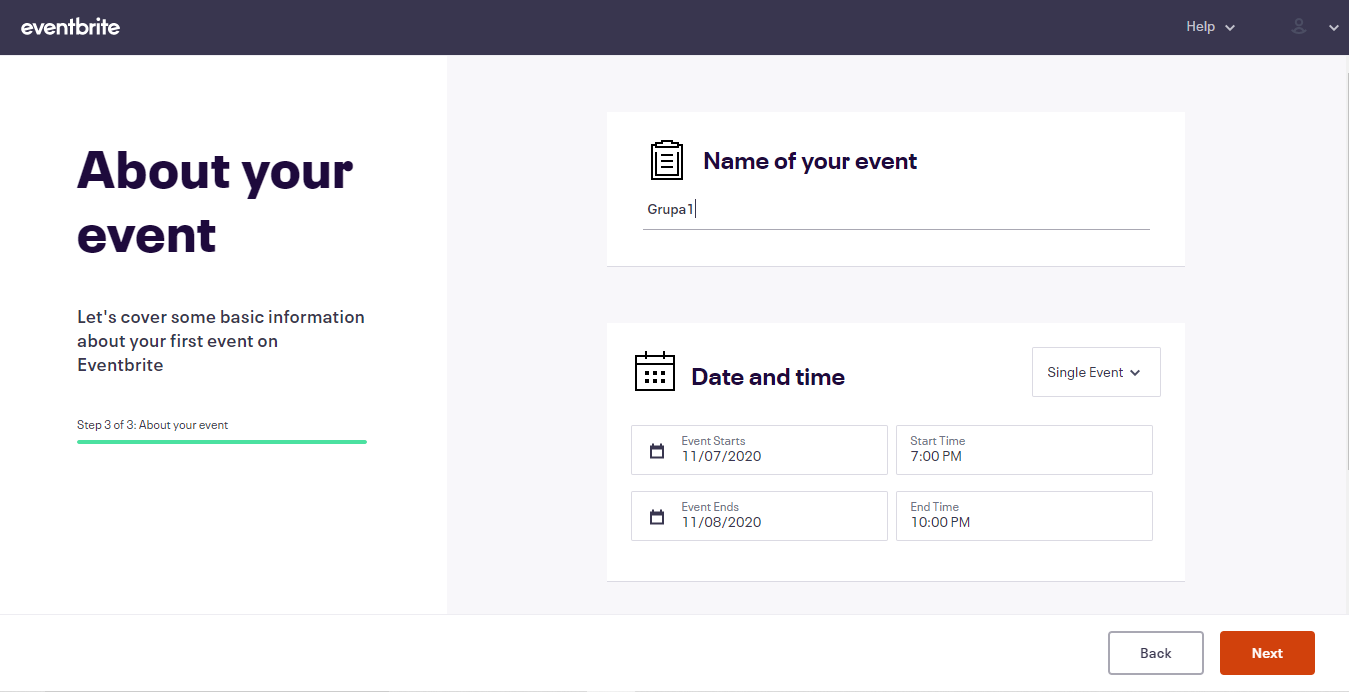
\includegraphics[width=.9\linewidth]{slike/eventbrite.png} %veličina u odnosu na širinu linije
			\centering
			\caption{Izgled \textit{eventbrite} forme pri pravljenju događaja}
			\label{fig:eventbrite} %label mora biti drugaciji za svaku sliku
		\end{figure}
		
		Postoje i alternative \textit{Eventbritu} slične kvalitete poput web stranice \textit{Billetto} dostupne na \url{https://billetto.co.uk/}. Ovaj servis dodatno omogućava korisnicima da pretražuju sve događaje dotad napravljene na toj stranici. Prednost takvog pristupa za organizatore je da im je time događaj dodatno reklamiran.
		
		\begin{figure}[H]
			
\includegraphics[width=.9\linewidth]{slike/billetto.png} %veličina u odnosu na širinu linije
			\centering
			\caption{Pretraživanje događaja na web stranici \textit{Billetto}}
			\label{fig:Billetto} %label mora biti drugaciji za svaku sliku
		\end{figure}
	
		Nadalje, slična funkcionalnostima, iako tematski nešto udaljenija je aplikacija \textit{Eventee} dostupna na \url{https://eventee.co}. Ova aplikacija osmišljena je kako bi pomogla organizacijama u stvaranju događaja i upravljanju njihovim sudionicima. Dodatno, aplikacija organizatorima šalje statističke podatke o događaju u stvarnom vremenu. 
		
		
		\begin{figure}[H]
			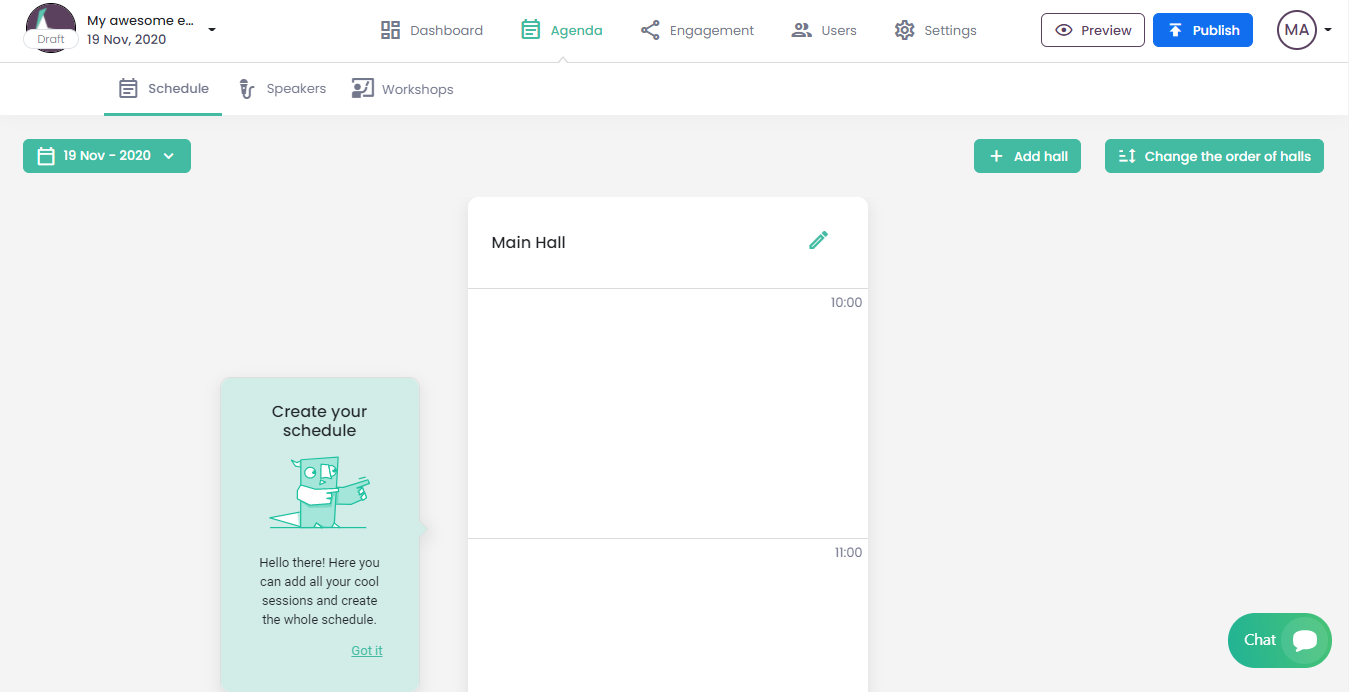
\includegraphics[width=.9\linewidth]{slike/eventee.png} %veličina u odnosu na širinu linije
			\centering
			\caption{Stvaranje novog događaja na web stranici \textit{Eventee}}
			\label{fig:eventee} %label mora biti drugaciji za svaku sliku
		\end{figure}
	
		Konačno, naveden je kratki pregled aplikacije \textit{Cvent} dostupe na \url{https://www.cvent.com}. Ova aplikacija nudi jednostavna i integrirana tehnološka rješenja kojima se nastoji maksimizirati učinak sastanaka i događaja različith veličina. Nastojanjem da povratnim informacijama o reakciji publike pomogne organizacijama u planiranju događaja kojima se cilja na određeno tržište, aplikacija se više orijentira na rješenja primjerena za događaje iz područja marketinga.  
		
		\begin{figure}[H]
			
\includegraphics[width=.9\linewidth]{slike/cvent.png} %veličina u odnosu na širinu linije
			\centering
			\caption{Početna stranica aplikacije \textit{Cvent}}
			\label{fig:cvent} %label mora biti drugaciji za svaku sliku
		\end{figure}
	
	
	
		
		\eject
		
		
		
		
	
	\chapter{Specifikacija programske potpore}
		
		\section{Funkcionalni zahtjevi}
	
	Aktori koji izravno komuniciraju sa sustavom mogu imati ulogu inicijatora ili sudionika.
	Inicijatori pokreću procese u sustavu, konkretno radi se o neregistriranom i registriranom korisniku, recenzentu, organizatoru konferencije i administratoru. S druge strane, sudionici obavljaju određene poslove, konkretno radi se o bazi podataka.
	\newline
	
	
	
	
	\noindent \textbf{Dionici:}
	
	\begin{packed_enum}
		
		\item Organizator konferencije
		\item Sudionik konferencije
		\item Recenzent
		\item Administrator
		\item Razvojni tim
		
	\end{packed_enum}
	
	\noindent \textbf{Aktori i njihovi funkcionalni zahtjevi:}
	
	
	\begin{packed_enum}
		
			\item  \underbar{Organizator konferencije (inicijator) može:}
		\begin{packed_enum}
			
			\item pregledati sve podatke o sudionicima te ih mijenjati i dodavati sadržaj
			\item sudionicima slati obavijesti na njihove adrese elektroničke pošte
			\item pohraniti na lokalno računalo sve pristigle radove
			
		\end{packed_enum}
		
		\item  \underbar{Registrirani korisnik (inicijator) može:}
		\begin{packed_enum}
			
			\item obaviti prijavu u sustav
			\item pregledati sve definirane konferencije i njihove sekcije
			\item odabrati sekciju u kojoj želi sudjelovati i obaviti prijavu na sekciju
			\item pohraniti i uređivati vlastiti rad
			\item pregledati i uređivati osobne podatke
			\item prijaviti se za recenzenta konferencije
			\item izbrisati svoj korisnički račun
			
		\end{packed_enum}
		
		\item  \underbar{Administrator (inicijator) može:}
		
		\begin{packed_enum}
			
			\item upisati podatke o konferenciji i odrediti organizatora konferencije
			\item pregledati i izmijeniti podatke registriranog korisnika
			\item pohraniti sve dokumente koje su sudionici poslali
			i potvrdili kao konačnu inačicu
			\item pregledati statistiku vezanu za korisnike:
			\begin{packed_enum}
				
				\item broj trenutno prijavljenih korisnika
				\item ukupan broj i imena svih registriranih korisnika\newline
				
			\end{packed_enum}
				
		\end{packed_enum}
		
		
		\item  \underbar{Recenzent (inicijator) može:}
		\begin{packed_enum}
			
			\item pregledati prispjele radove svih sudionika konferencije
			\item definirati recenziju rada i odgovor na korisnikov zahtjev za sudjelovanjem na konferenciji: 
			\begin{packed_enum}
				
				\item prihvaćanjem rada
				\item prihvaćanjem rada, ali uz potrebnu doradu u manjoj mjeri
				(nije potrebna naknadna provjera)
				\item prihvaćanjem rada, ali uz potrebnu doradu u većoj mjeri
				(potrebna naknadna provjera)
				\item odbijanjem rada uz navođenje valjanog razloga
				
			\end{packed_enum}
			
			
		\end{packed_enum}
	
			\item  \underbar{Neregistrirani/neprijavljeni korisnik (inicijator) može:}
		\begin{packed_enum}
			
			\item obaviti registraciju u sustav, stvoriti novi korisnički račun za koji su mu potrebni ime, prezime, naziv institucije ili poduzeća u kojem djeluje, adresa boravka i adresa elektroničke pošte 
			
		\end{packed_enum}
		
		\item  \underbar{Baza podataka (sudionik):}
		
		\begin{packed_enum}
			
			\item pohranjuje podatke o svim korisnicima i njihovim ovlastima
			\item pohranjuje sve podatke o konferencijama, njihovim sekcijama i prispjelim radovima
			
			
		\end{packed_enum}
		
	
	\end{packed_enum}
	
	\eject 
	
			
			
				
			\subsection{Obrasci uporabe}
			
				
				\subsubsection{Opis obrazaca uporabe}
					

					\noindent \underbar{\textbf{UC1 - Registracija u sustav}}
					\begin{packed_item}
	
						\item \textbf{Glavni sudionik: }Neregistrirani korisnik
						\item  \textbf{Cilj:} Stvaranje korisničkog računa za pristup sustavu
						\item  \textbf{Sudionici:} Baza podataka
						\item  \textbf{Preduvjet:} -
						\item  \textbf{Opis osnovnog tijeka:}
						
						\item[] \begin{packed_enum}
							
							\item Korisnik odabire opciju za registraciju u sustav
							\item Korisnik unosi svoje podatke
							\item Korisniku se pridjeljuje njegova identifikacija
							\item Generira se lozinka koja se šalje korisniku
							\item Sustav šalje korisniku poveznicu za potvrdu registracije
							
						\end{packed_enum}
						
						\item  \textbf{Opis mogućih odstupanja:}
						
						\item[] \begin{packed_item}
	
							\item[2.a] Odabir već zauzetog korisničkog imena i/ili e-maila, unos korisničkih podataka u nedozvoljenom formatu ili pružanje neispravnog e-maila
							\item[] \begin{packed_enum}
								
								\item Sustav obavještava korisnika o neuspjelom upisu i vraća ga na stranicu za registraciju
								\item Korisnik mijenja potrebne podatke te završava unos ili odustaje od registracije
								
							\end{packed_enum}
						\end{packed_item}
					\end{packed_item}
				
				\noindent \underbar{\textbf{UC1.1 - Potvrdi registraciju}}
				\begin{packed_item}
					
					\item \textbf{Glavni sudionik: }Neregistrirani korisnik
					\item  \textbf{Cilj:} Potvrditi svoju registraciju u sustav
					\item  \textbf{Sudionici:} Baza podataka
					\item  \textbf{Preduvjet:} Ispunjen obrazac za uporabu
					\item  \textbf{Opis osnovnog tijeka:}
					
					\item[] \begin{packed_enum}
						
						\item Korisnik e-mailom prima poveznicu za potvrdu registracije
						\item Korisnik klikom na poveznicu potvrđuje stvaranje korisničkog računa
						\item Korisnikovi podatci se pohranjuju u bazu podataka
					
					\end{packed_enum}
					
					\item  \textbf{Opis mogućih odstupanja:}
					
					\item[] \begin{packed_item}
						
						\item[2.a] Korisnik ne potvrđuje svoju prijavu klikom na dobivenu poveznicu
						
						\item[] \begin{packed_enum}
							
							\item Registracija se ne potvrđuje\newline
							
						\end{packed_enum}
					\end{packed_item}
				\end{packed_item}
				
				\noindent \underbar{\textbf{UC2 - Pregled konferencija}}
				\begin{packed_item}
					
					\item \textbf{Glavni sudionik: }Registrirani korisnik
					\item  \textbf{Cilj:} Pregledati popis svih konferencija
					\item  \textbf{Sudionici:} Baza podataka
					\item  \textbf{Preduvjet:} Korisnik je prijavljen
					\item  \textbf{Opis osnovnog tijeka:}
					
					\item[] \begin{packed_enum}
						
						\item Korisnik odabire opciju "Pregledaj konferencije"
						\item Korisniku se prikazuju sve postojeće konferencije
						\item Korisnik odabire jednu od konferencija
						\item Prikazuju se informacije o konferenciji
						
					\end{packed_enum}
				\end{packed_item}
			
			\noindent \underbar{\textbf{UC3 - Prijava u sustav}}
			\begin{packed_item}
				
				\item \textbf{Glavni sudionik: }Registrirani korisnik
				\item  \textbf{Cilj:} Dobiti pristup početnom korisničkom sučelju i korisničkim funkcijama
				\item  \textbf{Sudionici:} Baza podataka
				\item  \textbf{Preduvjet:} Sudionik je registriran
				\item  \textbf{Opis osnovnog tijeka:}
				
				\item[] \begin{packed_enum}
					
					\item Korisnik izabire opciju "Prijava"
					\item Korisnik unosi svoj e-mail i lozinku
					\item Potvrda o ispravnosti unesenih podataka
					\item Pristup korisničkim funkcijama
					
				\end{packed_enum}
				
				\item  \textbf{Opis mogućih odstupanja:}
				
				\item[] \begin{packed_item}
					
					\item[3.a] Neispravno korisničko ime ili lozinka
					
					\item[] \begin{packed_enum}
						
						\item Sustav obavještava korisnika o neuspjeloj prijavi i vraća ga na stranicu za prijavu
						
					\end{packed_enum}
				\end{packed_item}
			\end{packed_item}
		
		\noindent \underbar{\textbf{UC3.1 - Generiranje nove lozinke}}
		\begin{packed_item}
			
			\item \textbf{Glavni sudionik: }Registrirani korisnik
			\item  \textbf{Cilj:} Dobiti novu lozinku na e-mail
			\item  \textbf{Sudionici:} Baza podataka
			\item  \textbf{Preduvjet:} Sudionik je registriran
			\item  \textbf{Opis osnovnog tijeka:}
			
			\item[] \begin{packed_enum}
				
				\item Korisnik odabire opciju "Zaboravljena lozinka"
				\item Korisnik u polje unosi svoju e-mail adresu
				\item Korisnik odabire gumb "Pošalji novu lozinku"
				\item Korisniku na e-mail dolazi nova lozinka za njegov račun
				
			\end{packed_enum}
			
			\item  \textbf{Opis mogućih odstupanja:}
			
			\item[] \begin{packed_item}
				
				\item[2.a] Neispravno unesena e-mail adresa
				
				\item[] \begin{packed_enum}
					
					\item Sustav obavještava korisnika da provjeri unesenu adresu
					
				\end{packed_enum}
			\end{packed_item}
		\end{packed_item}
	
	\noindent \underbar{\textbf{UC4 - Prijava za sudjelovanje na konferenciji}}
	\begin{packed_item}
		
		\item \textbf{Glavni sudionik: }Registrirani korisnik
		\item  \textbf{Cilj:} Prijaviti se na željenu konferenciju
		\item  \textbf{Sudionici:} Baza podataka
		\item  \textbf{Preduvjet:} Korisnik je prijavljen, postoje definirane konferencije
		\item  \textbf{Opis osnovnog tijeka:}
		
		\item[] \begin{packed_enum}
			
			\item  Korisnik bira opciju "Prijava za sudjelovanje na konferenciji"
			\item Korisniku se prikazuje lista svih postojećih konferencija
			\item Korisnik odabire konferenciju
			\item Korisniku se prikazuju informacije o konferenciji i popis sekcija
			\item Korisnik izabire opciju "Prijavi se"
			\item Korisniku se otvara obrazac za prijavu kojeg popunjava
			\item Korisnik potvrđuje prijavu
			
		\end{packed_enum}
	\end{packed_item}

	\noindent \underbar{\textbf{UC4.1 - Odabir sekcije}}
	\begin{packed_item}
		
		\item \textbf{Glavni sudionik: }Registrirani korisnik
		\item  \textbf{Cilj:} Odabrati sekciju unutar konferencije
		\item  \textbf{Sudionici:} Baza podataka
		\item  \textbf{Preduvjet:} Korisnik je prijavljen, nije prošao datum za prijavu u sekciju
		\item  \textbf{Opis osnovnog tijeka:}
		
		\item[] \begin{packed_enum}
			
			\item  Korisniku je prikazana lista sekcija koje može odabrati
			\item Korisnik odabire željenu sekciju
			
		\end{packed_enum}
	\end{packed_item}

	\noindent \underbar{\textbf{UC4.2 - Slanje potvrde o uspješnoj prijave}}
	\begin{packed_item}
		
		\item \textbf{Glavni sudionik: }Registrirani korisnik
		\item  \textbf{Cilj:} Dobiti odobrenje za sudjelovanje na konferenciji
		\item  \textbf{Sudionici:} Baza podataka
		\item  \textbf{Preduvjet:} Korisnik je prijavljen
		\item  \textbf{Opis osnovnog tijeka:}
		
		\item[] \begin{packed_enum}
			
			\item  Korisnik na e-mail dobiva potvrdu za sudjelovanje u sekciji
			\item Određuje se vrijeme unutar kojeg korisnik mora učitati svoj rad
			
		\end{packed_enum}
	\end{packed_item}

	\noindent \underbar{\textbf{UC4.3 - Učitavanje rada}}
	\begin{packed_item}
		
		\item \textbf{Glavni sudionik: }Registrirani korisnik
		\item  \textbf{Cilj:} Učitati svoj rad
		\item  \textbf{Sudionici:} Baza podataka
		\item  \textbf{Preduvjet:} Korisnik je prijavljen u sustav; odobrena mu je prijava u sekciju; nije prošlo vrijeme za učitavanje rada
		\item  \textbf{Opis osnovnog tijeka:}
		
		\item[] \begin{packed_enum}
			
			\item  Korisnik odabire opciju "Učitaj svoj rad"
			\item Korisniku se otvara polje u koje može učitati rad
			\item Korisnik odabire gumb "Pošalji" za slanje rada
			\item Sustav korisniku šalje obavijest o primitku rada
			
		\end{packed_enum}
		
		\item  \textbf{Opis mogućih odstupanja:}
		
		\item[] \begin{packed_item}
			
			\item[2.a] Korisnik je učitao datoteku koja nije u pdf formatu
			\item[] \begin{packed_enum} 
				\item Korisniku se javlja da je učitao datoteku pogrešnog formata
					\end{packed_enum}
				
			\item[2.b] Korisnik nije stisnuo gumb za slanje rada
			\item[] \begin{packed_enum}
				\item Sustav javlja korisniku da nije poslao učitani rad
				
			\end{packed_enum}
		\end{packed_item}
	\end{packed_item}

	\noindent \underbar{\textbf{UC5 - Pregled osobnih podataka}}
	\begin{packed_item}
		
		\item \textbf{Glavni sudionik: }Registrirani korisnik
		\item  \textbf{Cilj:} Pregledati osobne podatke
		\item  \textbf{Sudionici:} Baza podataka
		\item  \textbf{Preduvjet:} Korisnik je prijavljen
		\item  \textbf{Opis osnovnog tijeka:}
		
		\item[] \begin{packed_enum}
			
			\item  Korisnik odabire opciju za pregled osobnih podataka
			\item Sustav prikazuje osobne podatke korisnika
			
		\end{packed_enum}
	\end{packed_item}

	\noindent \underbar{\textbf{UC6 - Uređivanje osobnih podataka}}
	\begin{packed_item}
		
		\item \textbf{Glavni sudionik: }Registrirani korisnik
		\item  \textbf{Cilj:} Urediti osobne podatke
		\item  \textbf{Sudionici:} Baza podataka
		\item  \textbf{Preduvjet:} Korisnik je prijavljen
		\item  \textbf{Opis osnovnog tijeka:}
		
		\item[] \begin{packed_enum}
			
			\item  Korisnik odabire opciju za promjenu osobnih podataka
			\item Korisnik mijenja svoje podatke
			\item Korisnik sprema promjene
			\item Baza podataka se ažurira
			
		\end{packed_enum}
		
		\item  \textbf{Opis mogućih odstupanja:}
		
		\item[] \begin{packed_item}
			
			\item[2.a] Korisnik promijeni osobne podatke, ali ne odabire opciju "Spremi promjene"
			\item[] \begin{packed_enum}
				
				\item Sustav obavještava korisnika da nije spremio podatke prije izlaska iz prozora
				
			\end{packed_enum}
		\end{packed_item}
	\end{packed_item}

	\noindent \underbar{\textbf{UC7 - Brisanje korisničkog računa}}
	\begin{packed_item}
		
		\item \textbf{Glavni sudionik: }Registrirani korisnik
		\item  \textbf{Cilj:} Izbrisati svoj korisnički račun
		\item  \textbf{Sudionici:} Baza podataka
		\item  \textbf{Preduvjet:} Korisnik je prijavljen
		\item  \textbf{Opis osnovnog tijeka:}
		
		\item[] \begin{packed_enum}
			
			\item  Korisnik odabire pregled osobnih podataka
			\item Otvara se stranica s osobnim podatcima
			\item Korisnik bira opciju za brisanje računa
			\item Korisnički račun se briše iz baze podataka
			\item Otvara se stranica za registraciju
			
		\end{packed_enum}
	\end{packed_item}

	\noindent \underbar{\textbf{UC8 - Prijava za recenziranje}}
	\begin{packed_item}
		
		\item \textbf{Glavni sudionik: }Registrirani korisnik
		\item  \textbf{Cilj:} Prijaviti se za ulogu recenzenta
		\item  \textbf{Sudionici:} Baza podataka
		\item  \textbf{Preduvjet:} Korisnik je prijavljen
		\item  \textbf{Opis osnovnog tijeka:}
		
		\item[] \begin{packed_enum}
			
			\item  Korisnik izabire opciju "Prijavi se za recenziranje"
			\item Korisniku se otvara obrazac za prijavu
			\item Korisnik ispunjava obrazac za prijavu i potvrđuje ga
			\item Nakon potvrde organizatora korisnik dobiva ovlasti recenzenta
			
		\end{packed_enum}
		
		\item  \textbf{Opis mogućih odstupanja:}
		
		\item[] \begin{packed_item}
			
			\item[4.a] Organizator konferencije odbija prijavu za recenziranje
			\item[] \begin{packed_enum}
				
				\item Korisnik dobiva obavijest o neuspješnoj potvrdi prijave
				
			\end{packed_enum}
		\end{packed_item}
	\end{packed_item}

	\noindent \underbar{\textbf{UC9 - Uredi učitani rad}}
	\begin{packed_item}
		
		\item \textbf{Glavni sudionik: }Registrirani korisnik
		\item  \textbf{Cilj:} Urediti svoj učitani rad
		\item  \textbf{Sudionici:} Baza podataka
		\item  \textbf{Preduvjet:} Korisnik je prijavljen, rad je prethodno učitan
		\item  \textbf{Opis osnovnog tijeka:}
		
		\item[] \begin{packed_enum}
			
			\item Korisnik odabire opciju "Uredi rad"
			\item Sustav prikazuje sve do tada predane radove
			\item Korisnik odabire rad koji želi urediti
			\item Korisnik uređuje rad
			\item Korisnik pohranjuje promjene
			\item Promjena se sprema u bazu podataka
		\end{packed_enum}
		
		\item  \textbf{Opis mogućih odstupanja:}
		
		\item[] \begin{packed_item}
			
			\item[2.a] Korisnik nema učitanih radova
			\item[] \begin{packed_enum}
				\item Sustav ispisuje poruku "Nema učitanih radova"
			
			\end{packed_enum}
	
			\item[4.a] Korisnik promijeni rad, ali ne odabire opciju "Spremi promjene"
			\item[] \begin{packed_enum}
				\item Sustav obavještava korisnika da nije spremio promjene prije izlaska iz prozora
			
			\end{packed_enum}
		\end{packed_item}
	\end{packed_item}

	\noindent \underbar{\textbf{UC10 - Pregledaj radove}}
	\begin{packed_item}
		
		\item \textbf{Glavni sudionik: }Recenzent
		\item  \textbf{Cilj:} Pregledati popis svih radova
		\item  \textbf{Sudionici:} Baza podataka
		\item  \textbf{Preduvjet:} Recenzent je prijavljen
		\item  \textbf{Opis osnovnog tijeka:}
		
		\item[] \begin{packed_enum}
			
			\item  Recenzent bira opciju "Pregledaj radove"
			\item Recenzentu se otvara popis svih učitanih radova
			
		\end{packed_enum}
		
		\item  \textbf{Opis mogućih odstupanja:}
		
		\item[] \begin{packed_item}
			
			\item[2.a] U sustav još nisu učitani radovi za odabranu sekciju
			\item[] \begin{packed_enum}
				
				\item Sustav ispisuje poruku "Nema radova"
				
			\end{packed_enum}
		\end{packed_item}
	\end{packed_item}

	\noindent \underbar{\textbf{UC11 - Prijava za sudjelovanje na konferenciji}}
	\begin{packed_item}
		
		\item \textbf{Glavni sudionik: }Recenzent
		\item  \textbf{Cilj:} Odbijanje rada
		\item  \textbf{Sudionici:} Baza podataka
		\item  \textbf{Preduvjet:} Recenzent je prijavljen, sudionik konferencije je učitao svoj rad
		\item  \textbf{Opis osnovnog tijeka:}
		
		\item[] \begin{packed_enum}
			
			\item  Recenzent bira opciju "Recenziraj rad"
			\item Recenzent bira ocjenu "Rad odbijen"
			\item Korisnik odabire konferenciju
			\item Recenzent unosi primjedbe u odgovarajuće polje
			\item Recenzent potvrđuje svoj odabir
			\item Sustav obavještava korisnika o odluci recenzenta
			
		\end{packed_enum}
	\end{packed_item}

	\noindent \underbar{\textbf{UC12 - Prihvati rad}}
	\begin{packed_item}
		
		\item \textbf{Glavni sudionik: }Recenzent
		\item  \textbf{Cilj:} Prihvatiti rad bez izmjena
		\item  \textbf{Sudionici:} Baza podataka
		\item  \textbf{Preduvjet:} Recenzent je prijavljen, sudionik konferencije je učitao svoj rad
		\item  \textbf{Opis osnovnog tijeka:}
		
		\item[] \begin{packed_enum}
			
			\item  Recenzent bira opciju "Recenziraj rad"
			\item Recenzent bira ocjenu "Rad prihvaćen"
			\item Recenzent potvrđuje svoj odabir
			\item Sustav obavještava korisnika o odluci recenzenta
			
		\end{packed_enum}
	\end{packed_item}

	\noindent \underbar{\textbf{UC13 - Prihvati rad uz izmjene}}
	\begin{packed_item}
		
		\item \textbf{Glavni sudionik: }Recenzent
		\item  \textbf{Cilj:} Izabrati željenu konferenciju
		\item  \textbf{Sudionici:} Baza podataka
		\item  \textbf{Preduvjet:} Recenzent je prijavljen, sudionik konferencije je učitao svoj rad
		\item  \textbf{Opis osnovnog tijeka:}
		
		\item[] \begin{packed_enum}
			
			\item Recenzent bira opciju "Recenziraj rad"
			\item Recenzent bira ocjenu "Rad prihvaćen uz izmjene"
			\item Recenzent unosi primjedbe u odgovarajuće polje
			\item Recenzent potvrđuje svoj odabir
			\item Sustav obavještava korisnika o odluci recenzenta
			
		\end{packed_enum}
	\end{packed_item}

	\noindent \underbar{\textbf{UC14 - Preuzmi rad lokalno}}
	\begin{packed_item}
		
		\item \textbf{Glavni sudionik: }Recenzent
		\item  \textbf{Cilj:} Preuzeti rad na svoje računalo
		\item  \textbf{Sudionici:} Baza podataka
		\item  \textbf{Preduvjet:} Recenzent je prijavljen, sudionik konferencije je učitao svoj rad
		\item  \textbf{Opis osnovnog tijeka:}
		
		\item[] \begin{packed_enum}
			
			\item Recenzent bira opciju "Preuzmi rad na računalo"
			\item Na računalo recenzenta se sprema rad u pdf formatu
			
		\end{packed_enum}
	\end{packed_item}

	\noindent \underbar{\textbf{UC15 - Pregledaj rad online}}
	\begin{packed_item}
		
		\item \textbf{Glavni sudionik: }Recenzent
		\item  \textbf{Cilj:} Pregledati rad online
		\item  \textbf{Sudionici:} Baza podataka
		\item  \textbf{Preduvjet:} Recenzent je prijavljen, sudionik konferencije je učitao svoj rad
		\item  \textbf{Opis osnovnog tijeka:}
		
		\item[] \begin{packed_enum}
			
			\item  Recenzent bira opciju "Pregledaj rad online"
			\item Rad se prikazuje u novoj kartici preglednika
			
		\end{packed_enum}
	\end{packed_item}

	\noindent \underbar{\textbf{UC16 - Odobri prijavu za recenziranje}}
	\begin{packed_item}
		
		\item \textbf{Glavni sudionik: }Organizator konferencije
		\item  \textbf{Cilj:} Odobriti zahtjev za recenziranje radova
		\item  \textbf{Sudionici:} Baza podataka
		\item  \textbf{Preduvjet:} Organizator je prijavljen
		\item  \textbf{Opis osnovnog tijeka:}
		
		\item[] \begin{packed_enum}
			
			\item Organizator konferencije odabire opciju "Zahtjevi za recenziranje"
			\item Sustav prikazuje popis primljenih zahtjeva za recenziranje
			\item Organizator konferencije odobrava ili odbacuje zahtjev
			\item Prijavljenog se obavještava o potvrđenoj prijavi
			
		\end{packed_enum}
		
		\item  \textbf{Opis mogućih odstupanja:}
		
		\item[] \begin{packed_item}
			
			\item[2.a] Nema primljenih zahtjeva za recenziranje
			\item[] \begin{packed_enum}
				
				\item Sustav ispisuje poruku "Nema pristiglih zahtjeva"
				
			\end{packed_enum}
		\end{packed_item}
	\end{packed_item}

	\noindent \underbar{\textbf{UC17 - Slanje obavijesti sudionicima}}
	\begin{packed_item}
		
		\item \textbf{Glavni sudionik: }Organizator konferencije
		\item  \textbf{Cilj:} Slanje obavijesti sudionicima
		\item  \textbf{Sudionici:} Baza podataka
		\item  \textbf{Preduvjet:} Organizator je prijavljen
		\item  \textbf{Opis osnovnog tijeka:}
		
		\item[] \begin{packed_enum}
			
			\item Organizator konferencije bira opciju "Pošalji obavijest sudionicima"
			\item Organizator konferencije upisuje obavijest u odgovarajuće polje
			\item Organizator odabire konferenciju među ponuđenima
			\item Sustav prikazuje popis svih sudionika za odabranu konferenciju
			\item Organizator konferencije bira opciju "Pošalji svima" ili odabire željene sudionike
			\item Potvrdom obavijesti ona se šalje sudionicima na e-mail
			
		\end{packed_enum}
		
		\item  \textbf{Opis mogućih odstupanja:}
		
		\item[] \begin{packed_item}
			
			\item[4.a] Na odabranoj konferenciji nema sudionika
			\item[] \begin{packed_enum}
				\item Sustav ispisuje poruku "Nema sudionika"
				
			\end{packed_enum}
			\item[6.a] Organizator sastavlja obavijest, ali napušta prozor bez potvrde slanja
			\item[] \begin{packed_enum}
				\item Sustav obavještava organizatora da slanje obavijesti nije potvrđeno
				
			\end{packed_enum}
		\end{packed_item}
	\end{packed_item}

	\noindent \underbar{\textbf{UC18 - Preuzmi rad sudionika}}
	\begin{packed_item}
		
		\item \textbf{Glavni sudionik: }Organizator konferencije
		\item  \textbf{Cilj:} Preuzeti pohranjeni rad sudionika konferencije
		\item  \textbf{Sudionici:} Baza podataka
		\item  \textbf{Preduvjet:} Organizator je prijavljen
		\item  \textbf{Opis osnovnog tijeka:}
		
		\item[] \begin{packed_enum}
			
			\item Organizator konferencije odabire opciju "Preuzmi rad sudionika"
			\item Prikazuje se popis svih radova po sekcijama
			\item Organizator odabire radove koje želi preuzeti
			\item Organizator potvrđuje odabir i radovi se preuzimaju
			
		\end{packed_enum}
		
		\item  \textbf{Opis mogućih odstupanja:}
		
		\item[] \begin{packed_item}
			
			\item[2.a] Nema učitanih radova na konfereniciji
			\item[] \begin{packed_enum}
				
				\item Sustav ispisuje poruku "Nema radova"
				
			\end{packed_enum}
		\end{packed_item}
	\end{packed_item}

	\noindent \underbar{\textbf{UC19 - Pregled statistike o radovima}}
	\begin{packed_item}
		
		\item \textbf{Glavni sudionik: }Organizator konferencije
		\item  \textbf{Cilj:} Pregledati broj radova ukupno i po sekcijama
		\item  \textbf{Sudionici:} Baza podataka
		\item  \textbf{Preduvjet:} Organizator je prijavljen
		\item  \textbf{Opis osnovnog tijeka:}
		
		\item[] \begin{packed_enum}
			
			\item Organizator odabire opciju "Pregledaj sve radove"
			\item Prikazuje se popis svih radova po sekcijama
			\item Organizator odabire opciju "Prikaži statistiku"
			\item Prikazuje se statistika za odabranu konferenciju
			
		\end{packed_enum}
	\end{packed_item}

	\noindent \underbar{\textbf{UC20 - Pregled podataka korisnika}}
	\begin{packed_item}
		
		\item \textbf{Glavni sudionik: }Administrator
		\item  \textbf{Cilj:} Pregledati podatke korisnika
		\item  \textbf{Sudionici:} Baza podataka
		\item  \textbf{Preduvjet:} Administrator je prijavljen
		\item  \textbf{Opis osnovnog tijeka:}
		
		\item[] \begin{packed_enum}
			
			\item Administrator bira opciju "Pregledaj podatke korisnika"
			\item Administrator konferencije pronalazi željenog sudionika
			\item Podatci korisnika se prikazuju
			
		\end{packed_enum}
		
		\item  \textbf{Opis mogućih odstupanja:}
		
		\item[] \begin{packed_item}
			
			\item[2.a] Nema registriranih korisnika
			\item[] \begin{packed_enum}
				
				\item Sustav ispisuje poruku "Nema registriranih korisnika"
				
			\end{packed_enum}
		\end{packed_item}
	\end{packed_item}

	\noindent \underbar{\textbf{UC21 - Mijenjanje podataka sudionika}}
	\begin{packed_item}
		
		\item \textbf{Glavni sudionik: }Administrator
		\item  \textbf{Cilj:} Promijeniti podatke sudioniku konferencije
		\item  \textbf{Sudionici:} Baza podataka
		\item  \textbf{Preduvjet:} Administrator je prijavljen
		\item  \textbf{Opis osnovnog tijeka:}
		
		\item[] \begin{packed_enum}
			
			\item Administrator bira opciju "Pregledaj podatke sudionika"
			\item Administrator pronalazi željenog sudionika
			\item Podatci korisnika se prikazuju
			\item Administrator bira opciju "Promijeni podatke"
			\item Administrator mijenja podatke sudioniku
			\item Administrator sprema promjene
			\item Baza podataka se ažurira
			
		\end{packed_enum}
		
		\item  \textbf{Opis mogućih odstupanja:}
		
		\item[] \begin{packed_item}
			
			\item[1.a] Nema registriranih korisnika
			\item[] \begin{packed_enum}
				\item Sustav ispisuje poruku "Nema registriranih korisnika"
				
			\end{packed_enum}
		
			\item[5.a] Organizator mijenja podatke, ali ne odabire opciju "Spremi promjene"
			\item[] \begin{packed_enum}
				\item Sustav obavještava organizatora da nije spremio podatke
				
			\end{packed_enum}
		\end{packed_item}
	\end{packed_item}

	\noindent \underbar{\textbf{UC22 - Dodavanje podataka sudioniku}}
	\begin{packed_item}
		
		\item \textbf{Glavni sudionik: }Administrator
		\item  \textbf{Cilj:} Dodati podatke sudioniku
		\item  \textbf{Sudionici:} Baza podataka
		\item  \textbf{Preduvjet:} Administrator je prijavljen
		\item  \textbf{Opis osnovnog tijeka:}
		
		\item[] \begin{packed_enum}
			
			\item Administrator bira opciju "Pregledaj podatke sudionika"
			\item Administrator pronalazi željenog sudionika
			\item Podatci korisnika se prikazuju
			\item Administrator bira opciju "Dodaj podatke"
			\item Administrator dodaje podatke sudioniku
			\item Administrator sprema promjene
			\item Baza podataka se ažurira
			
		\end{packed_enum}
		
		\item  \textbf{Opis mogućih odstupanja:}
		
		\item[] \begin{packed_item}
			
			\item[1.a] Nema registriranih korisnika
			\item[] \begin{packed_enum}
				\item Sustav ispisuje poruku "Nema registriranih korisnika"
				
			\end{packed_enum}
			
			\item[5.a] Organizator dodaje podatke, ali ne odabire opciju "Spremi promjene"
			\item[] \begin{packed_enum}
				\item Sustav obavještava organizatora da nije spremio podatke
				
			\end{packed_enum}
		\end{packed_item}
	\end{packed_item}

	\noindent \underbar{\textbf{UC23 - Pregled aktivnih korisnika}}
	\begin{packed_item}
		
		\item \textbf{Glavni sudionik: }Administrator
		\item  \textbf{Cilj:} Pregledati aktivne korisnike
		\item  \textbf{Sudionici:} Baza podataka
		\item  \textbf{Preduvjet:} Administrator je prijavljen
		\item  \textbf{Opis osnovnog tijeka:}
		
		\item[] \begin{packed_enum}
			
			\item Administrator odabire opciju "Popis aktivnih korisnika"
			\item Prikazuje se popis i broj korisnika koji su trenutno aktivni
			
		\end{packed_enum}
	\end{packed_item}

	\noindent \underbar{\textbf{UC24 - Stvaranje nove konferencije}}
	\begin{packed_item}
		
		\item \textbf{Glavni sudionik: }Administrator
		\item  \textbf{Cilj:} Stvoriti novu konferenciju
		\item  \textbf{Sudionici:} Baza podataka
		\item  \textbf{Preduvjet:} Administrator je prijavljen
		\item  \textbf{Opis osnovnog tijeka:}
		
		\item[] \begin{packed_enum}
			
			\item Administrator odabire opciju "Stvori novu konferenciju"
			\item Prikazuje se prozor za unos opcija
			\item Administrator popunjava opcije
			\item Administrator potvrđuje unesene podatke
			
		\end{packed_enum}
		
		\item  \textbf{Opis mogućih odstupanja:}
		
		\item[] \begin{packed_item}
			
			\item[1.a] Administrator dodaje podatke, ali ne odabire opciju "Spremi promjene"
			\item[] \begin{packed_enum}
				\item Sustav obavještava administratora da nije spremio podatke\newline\newline\newline
				
			\end{packed_enum}
		\end{packed_item}
	\end{packed_item}

	\noindent \underbar{\textbf{UC24.1 - Upisivanje podataka o konferenciji}}
	\begin{packed_item}
		
		\item \textbf{Glavni sudionik: }Administrator
		\item  \textbf{Cilj:} Upisati podatke za novu konferenciju
		\item  \textbf{Sudionici:} Baza podataka
		\item  \textbf{Preduvjet:} Administrator je prijavljen
		\item  \textbf{Opis osnovnog tijeka:}
		
		\item[] \begin{packed_enum}
			
			\item Administrator odabire opciju za unos podataka o konferenciji
			\item Administrator unosi sve potrebne podatke o konferenciji
			
		\end{packed_enum}
	\end{packed_item}

	\noindent \underbar{\textbf{UC24.2 - Odredi organizatora konferencije}}
	\begin{packed_item}
		
		\item \textbf{Glavni sudionik: }Administrator
		\item  \textbf{Cilj:} Odrediti organizatora nove konferencije
		\item  \textbf{Sudionici:} Baza podataka
		\item  \textbf{Preduvjet:} Administrator je prijavljen
		\item  \textbf{Opis osnovnog tijeka:}
		
		\item[] \begin{packed_enum}
			
			\item Administrator odabire opciju za dodavanje organizatora
			\item Administrator u sustavu odabire organizatora konferencije
			
		\end{packed_enum}
	\end{packed_item}

	\noindent \underbar{\textbf{UC24.3 - Definiranje upitnika za prijavu}}
	\begin{packed_item}
		
		\item \textbf{Glavni sudionik: }Administrator
		\item  \textbf{Cilj:} Definirati upitnik za prijavu na konferenciju
		\item  \textbf{Sudionici:} Baza podataka
		\item  \textbf{Preduvjet:} Administrator je prijavljen
		\item  \textbf{Opis osnovnog tijeka:}
		
		\item[] \begin{packed_enum}
			
			\item Administrator odabire opciju za definiranje upitnika za prijavu
			\item Administrator definira upitnik na temelju zahtjeva organizatora
			
		\end{packed_enum}
	\end{packed_item}
	
				\subsubsection{Dijagrami obrazaca uporabe}
				
				\begin{figure}[H]
					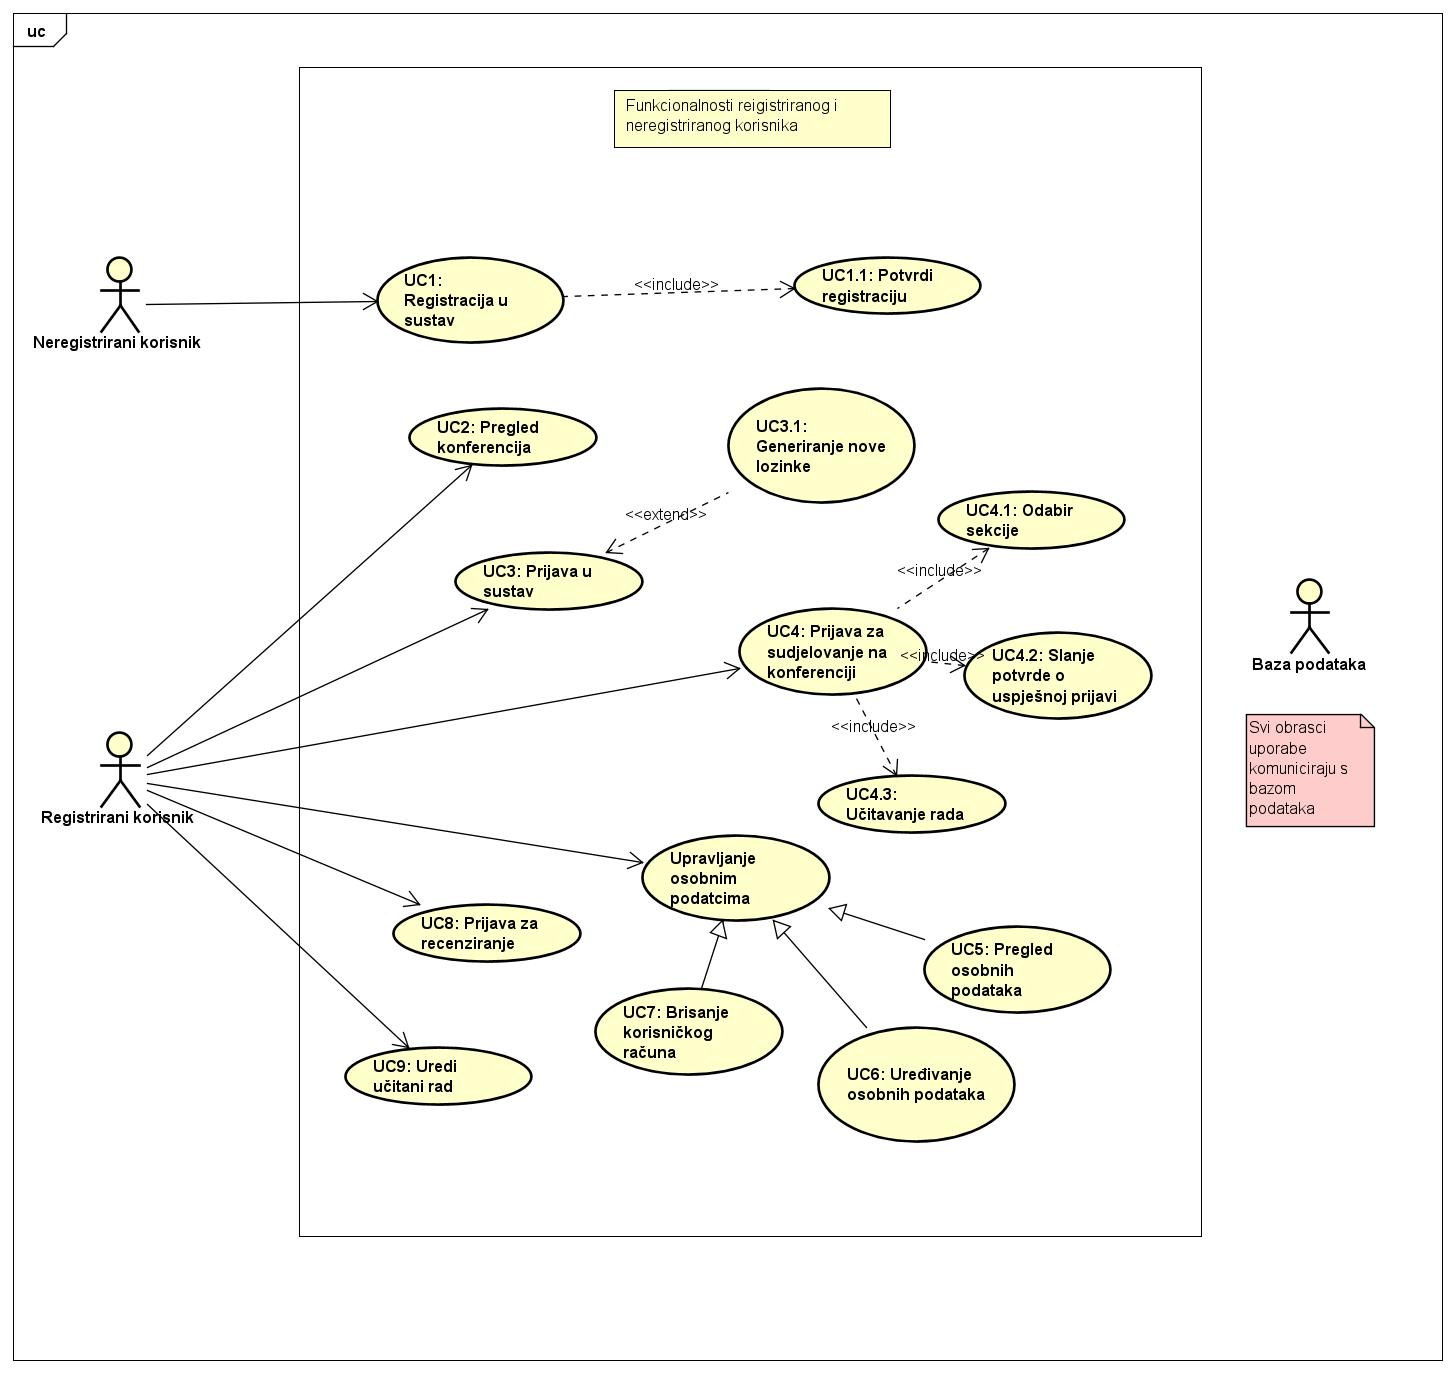
\includegraphics[width=1\linewidth]{slike/UCdijagram1} %veličina u odnosu na širinu linije
					\centering
					\caption{Dijagram obrasca uporabe, funkcionalnosti neregistriranog i registriranog korisnika}
					\label{fig:UC1} %label mora biti drugaciji za svaku sliku
				\end{figure}
			
				\begin{figure}[H]
					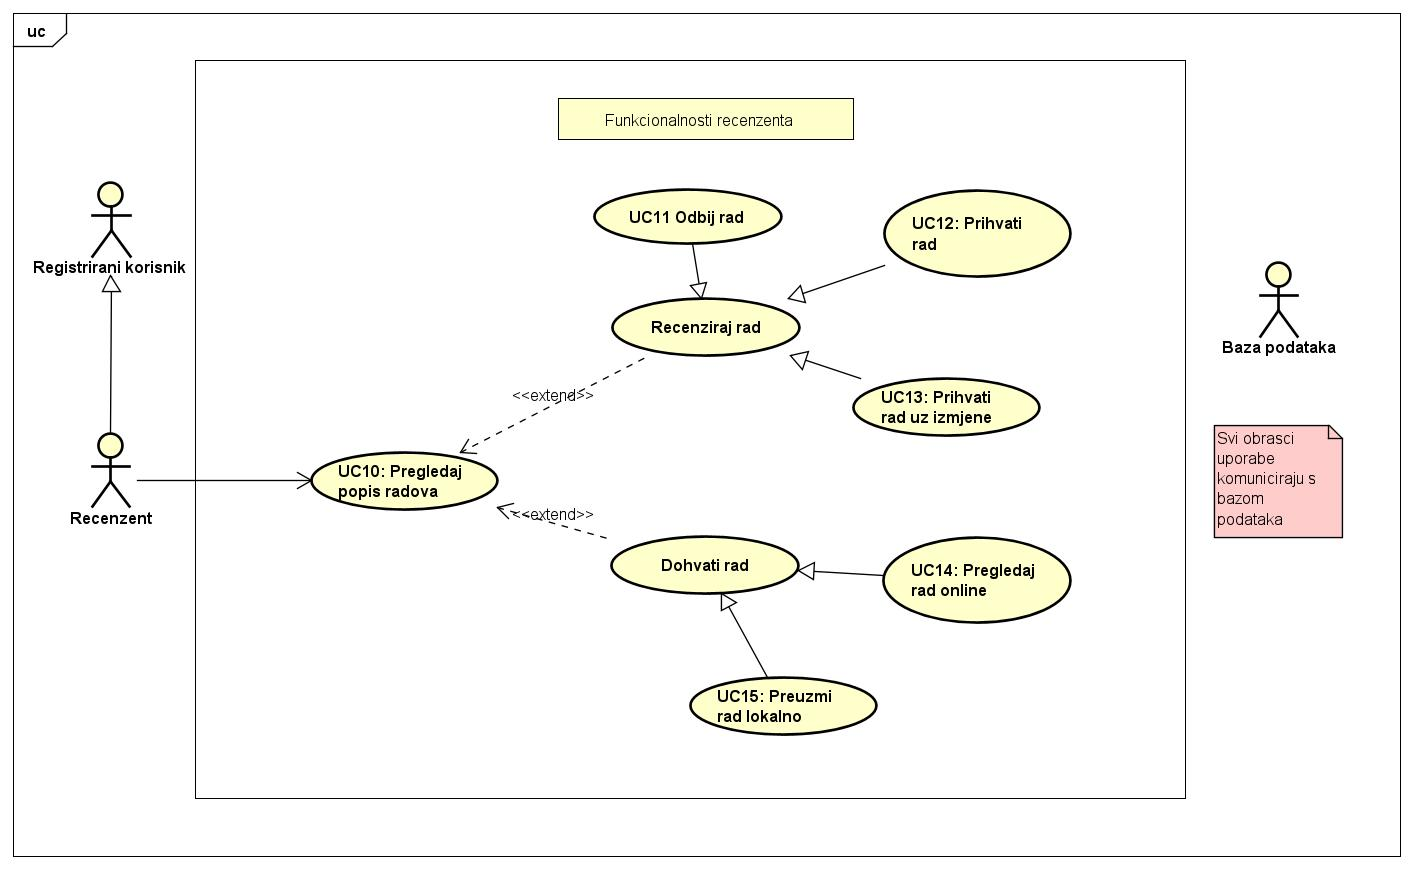
\includegraphics[width=1\linewidth]{slike/UCdijagram2} %veličina u odnosu na širinu linije
					\centering
					\caption{Dijagram obrasca uporabe, funkcionalnosti recenzenta}
					\label{fig:UC2} %label mora biti drugaciji za svaku sliku
				\end{figure}
				
				\begin{figure}[H]
					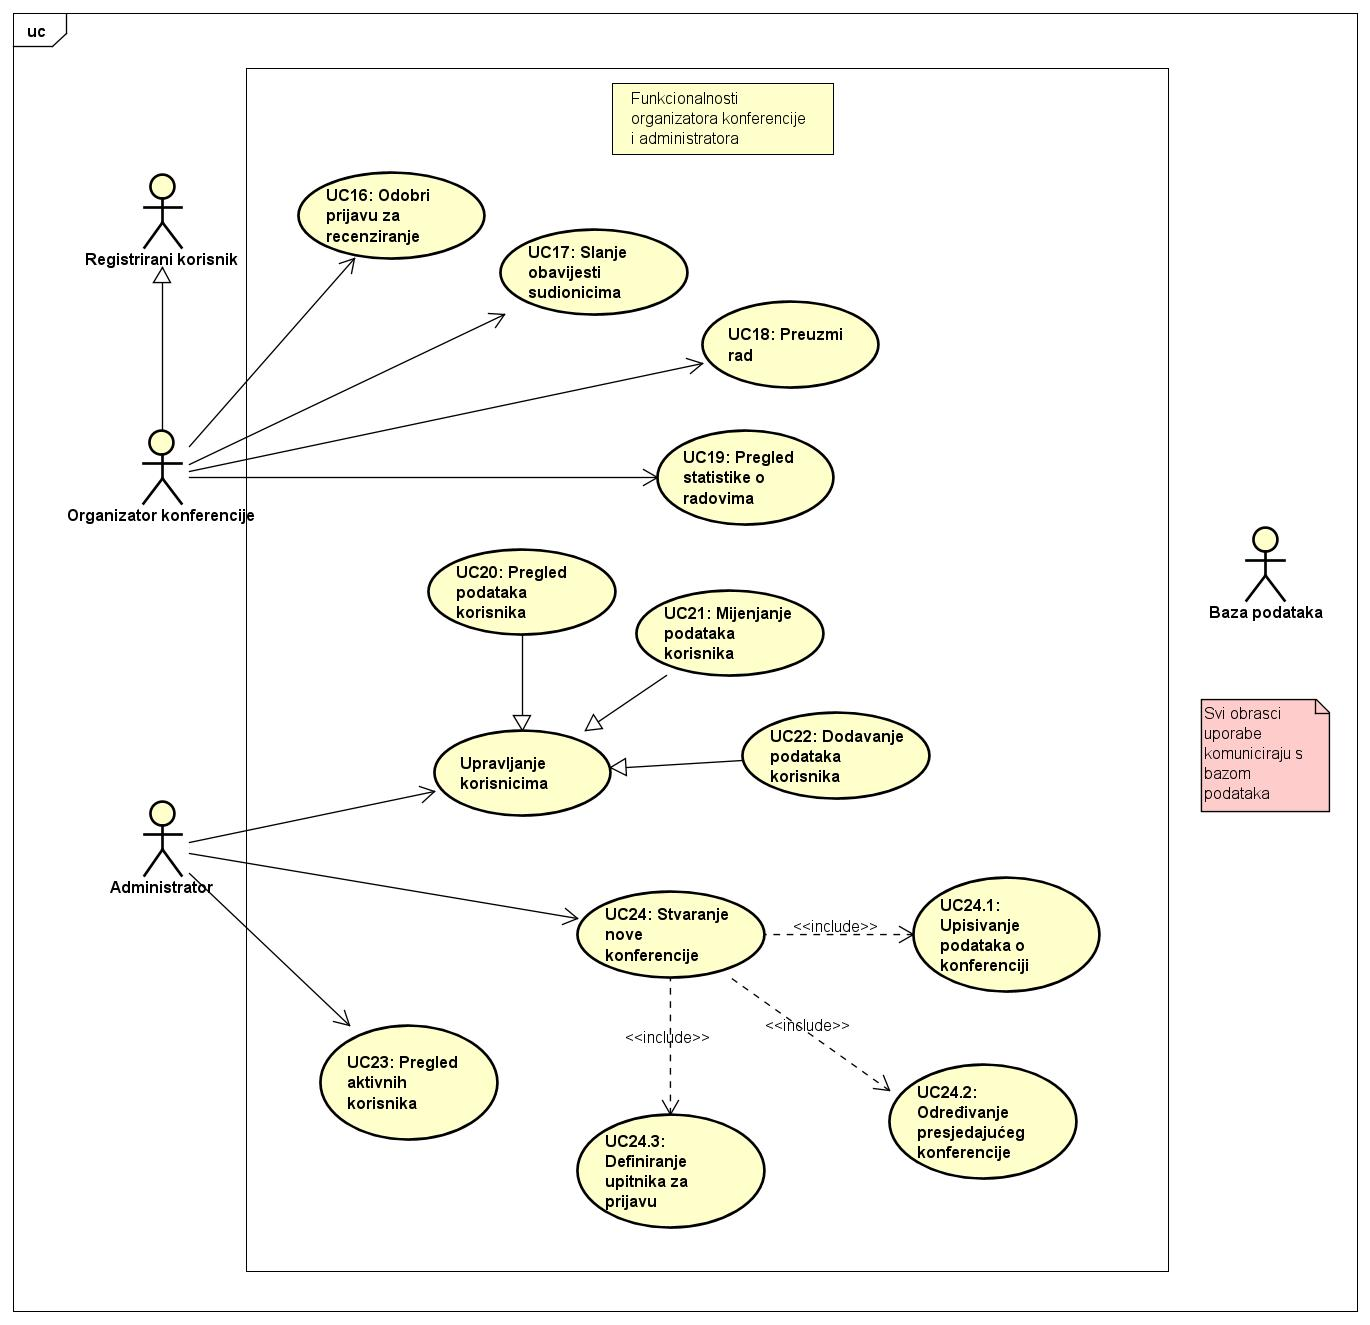
\includegraphics[width=1\linewidth]{slike/UCdijagram3} %veličina u odnosu na širinu linije
					\centering
					\caption{Dijagram obrasca uporabe, funkcionalnosti organizatora konferencije i administratora}
					\label{fig:UC3} %label mora biti drugaciji za svaku sliku
				\end{figure}
		
			\text\newline\newline\newline\newline\newline\newline
				
			\subsection{Sekvencijski dijagrami}

				
				\noindent\textbf{Obrazac uporabe UC6 - Uređivanje osobnih podataka}\\
				
				\noindent Korisnik odabire opciju za promjenu osobnih podataka. Poslužitelj iz baze podataka dohvaća osobne podatke korisnika postavljene pri obavljanju registracije u sustav i stvaranju korisničkog računa. Biranjem odabrane funkcionalnosti sustava i uspješnim dohvaćanjem osobnih podataka iz baze podataka korisnik dobiva pregled svih ranije definiranih osobnih podataka. Korisnik mijenja svoje podatke unošenjem novih vrijednosti te sprema promjene čime se baza podataka ažurira. Ukoliko korisnik nije spremio promjene sustav ga o tome obavještava.
				
				\begin{figure}[H]
					\includegraphics[width=1\linewidth]{slike/"UC6 sekvencijski"} %veličina u odnosu na širinu linije
					\centering
					\caption{Sekvencijski dijagram - Uređivanje osobnih podataka}
					\label{UC6 sekvencijski} %label mora biti drugaciji za svaku sliku
				\end{figure}
			
			
				\text\newline\newline\newline\newline\newline\newline\newline\newline\newline
			
				\noindent\textbf{Obrazac uporabe UC8 - Prijava za recenziranje}\\
				
				\noindent Korisnik na temelju popisa svih konferencija ranije definiranih u sustavu odabire konkretnu konferenciju na kojoj želi obavljati funkciju recenzenta radova sudionika konferencije. Korisnik šalje poslužitelju zahtjev za obrazac koji treba ispuniti kako bi izvršio prijavu. Sustav mu šalje unaprijed definirani obrazac za prijavu za recenziranje radova. Korisnik ispunjava obrazac svojim podacima i potvrđuje čime se njegovi podaci privremeno spremaju u bazu podataka. U slučaju potvrde od strane organizatora korisnik dobiva ovlasti recenzenta te se podaci trajno spremaju u bazi podataka. Ukoliko organizator odbije prijavu, korisnika se o tome obavještava.\newline\newline\newline\newline\newline
				
				\begin{figure}[H]
					\includegraphics[width=1\linewidth]{slike/"UC8 sekvencijski"} %veličina u odnosu na širinu linije
					\centering
					\caption{Sekvencijski dijagram - Prijava za recenziranje}
					\label{UC8 sekvencijski} %label mora biti drugaciji za svaku sliku
				\end{figure}
			
				\text\newline\newline\newline\newline\newline\newline\newline\newline\newline\newline\newline\newline\newline\newline
			
				\noindent\textbf{Obrazac uporabe UC9 - Uredi učitani rad}\\
				
				\noindent Korisnik na temelju poslanog zahtjeva za svim radovima pohranjenim u sklopu prijave za sudjelovanje na konferenciji dobiva pregled svih radova koje je do trenutka slanja upita poslužitelju pohranio u sustav. U suprotnom, ukoliko ranije nije pohranio niti jedan rad, tada sustav korisnika obavještava o nedostatku pohranjenih radova prikladnom porukom. Inače, odabirom jednog od ponuđenih radova, korisnik dobiva opciju uređivanja odabranog rada. Nakon što korisnik obavi uređivanje rada, ukoliko je pohranio promjene, iste se spremaju u bazu podataka, inače, ako nije spremio promjene prije izlaska, sustav ga o tome obavještava te traži potvrdu njegove odluke.
				
				\begin{figure}[H]
					\includegraphics[width=1\linewidth]{slike/"UC9 sekvencijski"} %veličina u odnosu na širinu linije
					\centering
					\caption{Sekvencijski dijagram - Uredi učitani rad}
					\label{UC9 sekvencijski} %label mora biti drugaciji za svaku sliku
				\end{figure}
				
				\text\newline\newline\newline\newline\newline\newline\newline\newline
	
		\section{Ostali zahtjevi}
		
			Zahtjevi kvalitete:
			 \begin{packed_item}
			 	\item Sustav treba omogućiti rad više korisnika u stvarnom vremenu
			 	\item Korisničko sučelje i sustav moraju podržavati hrvatsku abacedu (dijakritičke znakove) pri unosu i prikazu tekstualnog sadržaja
			 	\item Izvršavanje dijela programa u kojem se pristupa bazi podataka ne smije trajati duže od nekoliko sekundi
			 	\item Sustav treba biti implementiran kao web aplikacija koristeći objektno-orijentirane jezike
			 	\item Neispravno korištenje korisničkog sučelja ne smije narušiti funkcionalnost i rad sustava
			 	\item Nadogradnja sustava ne smije narušavati postojeće funkcionalnosti sustava
			 	\item Veza s bazom mora biti kvalitetno zaštićena, brza i otporna na vanjske greške
			 	\item Pristup sustavu mora biti omogućen iz javne mreže pomoću HTTPS
			 	
			 \end{packed_item}
	\text{\newline}	 
	 Ograničenja:
		 \begin{packed_item}
			 \item Nadogradnja sustava nije moguća bez izvornog koda i programskog jezika u kojem je aplikacija napisana
			 \item Veličina tekstualnog dokumenta ograničena je na 1 MB
			 \item Nije moguće pokrenuti dvije aplikacije, različitih korisnika s iste IP adrese
		\end{packed_item}
			 
	
	\chapter{Arhitektura i dizajn sustava}		

				
		\section{Baza podataka}
			
			\textit{Za potrebe našeg sustava koristit ćemo relacijsku bazu podataka koja svojom strukturom olakšava modeliranje znanstvene konferencije i njenih sudionika. Gradivna jedinka baze je relacija, odnosno tablica koja je definirana svojim imenom i skupom atributa. Zadaća baze podataka je brza i jednostavna pohrana, izmjena i dohvat podataka za daljnju obradu.
				Baza podataka ove aplikacije sastoji se od sljedećih entiteta:}
			
			\begin{itemize}
				\item 	\textit{Prijavljeni korisnik}
				\item 	\textit{Autor}
				\item 	\textit{Rad}
				\item 	\textit{Sekcija}
				\item 	\textit{Konferencija}
				\item 	\textit{Administrator}
				\item 	\textit{Organizator}
				\item 	\textit{Recenzent}		
			\end{itemize}
			
			\subsection{Opis tablica}
			
			
			\textbf{Prijavljeni korisnik}\space\space\space Ovaj entitet sadržava sve važne informacije o korisniku aplikacije.
				Sadrži atribute: Identifikacija, ime, prezime, adresa, naziv institucije/poduzeća, sekcija. Ovaj entitet u vezi je One-to-One s entitetom Rad preko atributa Identifikacija prijavljenog korisnika
			
			\begin{longtabu} to \textwidth {|X[6, l]|X[6, l]|X[20, l]|}
				
				\hline \multicolumn{3}{|c|}{\textbf{Prijavljeni korisnik}}	 \\[3pt] \hline
				\endfirsthead
				
				\hline \multicolumn{3}{|c|}{\textbf{Prijavljeni korisnik}}	 \\[3pt] \hline
				\endhead
				
				\hline 
				\endlastfoot
				
				\cellcolor{LightGreen} Identifikacija & INT	&  jedinstveni identifikator korisnika\\ \hline
				Ime	& VARCHAR & ime prijavljenog korisnika  	\\ \hline 
				Prezime & VARCHAR &  prezime prijavljenog korisnika \\ \hline 
				Adresa & VARCHAR	&  adresa stanovanja prijavljenog korisnika
				(ulica, kućni broj, grad, država)		\\ \hline 
				Naziv institucije poduzeća & VARCHAR	&  naziv institucije/poduzeća pod čijim pokroviteljstvom je rad proveden		\\ \hline 
				Sekcija & VARCHAR	& sekcija u koju se korisnik prijavljuje  		\\ \hline 
				Email & VARCHAR	& email adresa korisnika  		\\ \hline 
				
				
				
			\end{longtabu}
			
			
			\textbf{Autor}\space\space\space Ovaj entitet sadržava sve važne informacije o autoru nekog rada.
				Sadrži atribute: E-mail adresa, ime, prezime. Ovaj entitet u vezi je Many-to-Many s entitetom Rad
			
			
			\begin{longtabu} to \textwidth {|X[6, l]|X[6, l]|X[20, l]|}
				
				\hline \multicolumn{3}{|c|}{\textbf{Autor}}	 \\[3pt] \hline
				\endfirsthead
				
				\hline \multicolumn{3}{|c|}{\textbf{Autor}}	 \\[3pt] \hline
				\endhead
				
				\hline 
				\endlastfoot
				
				\cellcolor{LightGreen} Email adresa & VARCHAR	&  jedinstvena e-mail adresa autora\\ \hline
				Ime	& VARCHAR & ime autora  	\\ \hline 
				Prezime & VARCHAR &  prezime autora \\ \hline 
				
				
			\end{longtabu}
			
			\textbf{Rad}\space\space\space	Ovaj entitet sadržava sve važne informacije o radu predanom na konferenciju.
				Sadrži atribute: ID rada, naziv rada, identifikacija, naziv sekcije, ID konferencije. Ovaj entitet u vezi je One-to-One s entitetom Prijavljeni korisnik preko atributa Identifikacija prijavljenog korisnika, Many-to-Many s entitetom Autor te Many-to-One s entitetom Sekcija preko atributa naziv sekcije te atributa ID konferencije
			
			\begin{longtabu} to \textwidth {|X[6, l]|X[6, l]|X[20, l]|}
				
				\hline \multicolumn{3}{|c|}{\textbf{Rad}}	 \\[3pt] \hline
				\endfirsthead
				
				\hline \multicolumn{3}{|c|}{\textbf{Rad}}	 \\[3pt] \hline
				\endhead
				
				\hline 
				\endlastfoot
				
				\cellcolor{LightGreen} ID rada & INT	&  Jedinstveni identifikator rada\\ \hline
				Naziv rada	& VARCHAR & naziv rada  	\\ \hline
				Identifikacija & INT	&  jedinstveni identifikator korisnika
				(Prijavljeni korisnik.identifikacija)\\ \hline 
				\cellcolor{LightBlue} Naziv sekcije	& VARCHAR	&  naziv sekcije na koju je rad prijavljen
				(sekcija.naziv sekcije)		\\ \hline 
				\cellcolor{LightBlue} ID konferencije	& INT &  ID konferencije na čiju je sekciju rad prijavljen
				(konferencija.ID konferencije) 		\\ \hline 
				
				
				
			\end{longtabu}
			
			\textbf{Sekcija	}\space\space\space	Ovaj slabi entitet sadržava sve važne informacije o sekciji na nekoj konferenciji.
				Sadrži atribute: Naziv sekcije, ID konferencije. Ovaj entitet u vezi je Many-to-One s entitetom Konferencija preko atributa ID konferencije te u vezi One-to-Many s entitetom Rad preko atributa naziv sekcije te atributa ID konferencije
			
			\begin{longtabu} to \textwidth {|X[6, l]|X[6, l]|X[20, l]|}
				
				\hline \multicolumn{3}{|c|}{\textbf{Sekcija}}	 \\[3pt] \hline
				\endfirsthead
				
				\hline \multicolumn{3}{|c|}{\textbf{Sekcija}}	 \\[3pt] \hline
				\endhead
				
				\hline 
				\endlastfoot
				
				\cellcolor{LightGreen} Naziv sekcije & VARCHAR	&  Jedinstveni naziv sekcije 
				(jedinstven za ovu konferenciju)\\ \hline
				
				\cellcolor{LightGreen} ID konferencije	& INT &  ID konferencije na čiju je sekciju rad prijavljen
				(konferencija.ID konferencije) 		\\ \hline 
				
				
				
			\end{longtabu}
			
			\textbf{Konferencija}\space\space\space	Ovaj entitet sadržava sve važne informacije o konferenciji.
				Sadrži atribute: ID konferencije, naziv konferencije, datum održavanja. Ovaj entitet u vezi je One-to-Many s entitetom Sekcija preko atributa ID konferencije te u vezi Many-to-One s entitetom Administrator preko atributa ID administratora
			
			\begin{longtabu} to \textwidth {|X[6, l]|X[6, l]|X[20, l]|}
				
				\hline \multicolumn{3}{|c|}{\textbf{Konferencija}}	 \\[3pt] \hline
				\endfirsthead
				
				\hline \multicolumn{3}{|c|}{\textbf{Konferencija}}	 \\[3pt] \hline
				\endhead
				
				\hline 
				\endlastfoot
				
				\cellcolor{LightGreen} ID konferencije	& INT &  ID konferencije  		\\ \hline 
				
				Naziv konferencije	& VARCHAR & naziv konferencije  	\\ \hline
				
				Datum održavanja	& DATE & datum održavanja konferencije  	\\ \hline
				
				\cellcolor{LightBlue} ID administratora & INT	&  Jedinstveni ID administratora konferencije
				(administrator.ID administratora)\\ \hline
				
				
				
			\end{longtabu}
			
			\textbf{Administrator}\space\space\space	Ovaj entitet sadržava sve važne informacije o administratoru konferencije.
				Sadrži atribute: ID administratora, ime, prezime. Ovaj entitet u vezi je One-to-Many s entitetom Konferencija preko atributa ID administratora te u vezi One-to-One s entitetom Organizator preko atributa ID administratora
			
			\begin{longtabu} to \textwidth {|X[6, l]|X[6, l]|X[20, l]|}
				
				\hline \multicolumn{3}{|c|}{\textbf{Administrator}}	 \\[3pt] \hline
				\endfirsthead
				
				\hline \multicolumn{3}{|c|}{\textbf{Administrator}}	 \\[3pt] \hline
				\endhead
				
				\hline 
				\endlastfoot
				
				\cellcolor{LightGreen} ID
				administratora	& INT &  ID administratora \\ \hline 
				
				Ime	& VARCHAR & ime administratora\\ \hline
				
				Prezime	& VARCHAR & prezime administratora 	\\ \hline
				
				
			\end{longtabu}
			
			\textbf{Organizator	}\space\space\space	Ovaj entitet sadržava sve važne informacije o organizatoru konferencije.
				Sadrži atribute: ID organizatora, ime, prezime, ID administratora. Ovaj entitet u vezi je One-to-Many s entitetom Recenzent preko atributa ID organizatora te u vezi One-to-One s entitetom Administrator preko atributa ID administratora
			
			\begin{longtabu} to \textwidth {|X[6, l]|X[6, l]|X[20, l]|}
				
				\hline \multicolumn{3}{|c|}{\textbf{Organizator}}	 \\[3pt] \hline
				\endfirsthead
				
				\hline \multicolumn{3}{|c|}{\textbf{Organizator}}	 \\[3pt] \hline
				\endhead
				
				\hline 
				\endlastfoot
				
				\cellcolor{LightGreen} ID
				organizatora & INT &  ID organizatora\\ \hline 
				
				Ime	& VARCHAR & ime organizatora\\ \hline
				
				Prezime	& VARCHAR & prezime organizatora 	\\ \hline
				
				\cellcolor{LightBlue} ID
				administratora	& INT &  ID administratora
				(administrator.ID administratora) \\ \hline 
				
				
			\end{longtabu}
			
			\textbf{Recenzent}\space\space\space	Ovaj entitet sadržava sve važne informacije o recenzentu.
				Sadrži atribute: ID recenzenta, ime, prezime, ID organizatora. Ovaj entitet u vezi je Many-to-Many s entitetom Rad te u vezi Many-to-One s entitetom Organizator preko atributa ID organizatora
			
			\begin{longtabu} to \textwidth {|X[6, l]|X[6, l]|X[20, l]|}
				
				\hline \multicolumn{3}{|c|}{\textbf{Recenzent}}	 \\[3pt] \hline
				\endfirsthead
				
				\hline \multicolumn{3}{|c|}{\textbf{Recenzent}}	 \\[3pt] \hline
				\endhead
				
				\hline 
				\endlastfoot
				
				\cellcolor{LightGreen} ID
				recenzenta & INT &  ID recenzenta\\ \hline 
				
				Ime	& VARCHAR & ime recenzenta\\ \hline
				
				Prezime	& VARCHAR & prezime recenzenta 	\\ \hline
				
				\cellcolor{LightBlue} ID
				organizatora	& INT &  ID organizatora
				(organizator.ID organizatora) \\ \hline 
				
				
			\end{longtabu}
			
			
			\subsection{Dijagram baze podataka}
			
			\begin{figure}[H]
				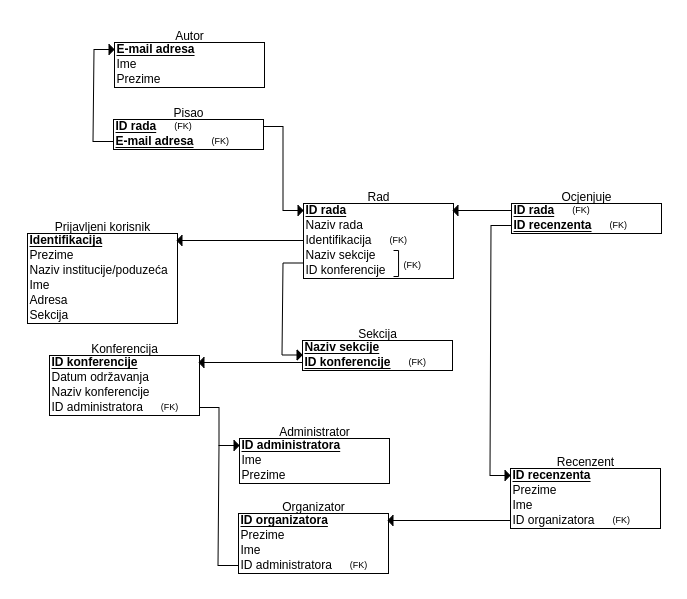
\includegraphics[width=.9\linewidth]{slike/ERdijagram.png} %veličina u odnosu na širinu linije
				\centering
				\caption{Relacijska shema baze podataka}
				\label{fig:RelShema} %label mora biti drugaciji za svaku sliku
			\end{figure}
			
			\eject
			
			
			
			
			
		\section{Dijagram razreda}
		
			\noindent \underbar{\textbf{Opis dijagrama razreda:}}
			\begin{packed_item}
				\item \textbf{Konferencija} Središnji razred koji predstavlja konferenciju
				\item \textbf{Administrator} Predstavlja administratora sustava, ima na raspolaganju sljedeći skup funkcionalnosti sustava:
				\begin{packed_item}
					\item Stvaranje nove konferencije
					\item Pregled statističkih podataka o korisnicima
					\item Izmjenu podataka registriranih korisnika
					\item Određivanje organizatora konferencije
				\end{packed_item}
				\item \textbf{Sekcija}  Konkretna sekcija na nekoj od konferencija
				\item \textbf{Recenzent} Predstavlja recenzenta na konferenciji, može pregledavati, \linebreak ocjenjivati i preuzimati radove na svoje računalo
				\item \textbf{Sudionik konferencije} Predstavlja sudionika na konferenciji,  omogućavaju \linebreak mu se sljedeće akcije:
				\begin{packed_item}
					\item Prijava na konferenciju
					\item Izmjena vlastitih podataka te promjena lozinke
					\item Učitavanje rada u pdf formatu
				\end{packed_item}
				\item \textbf{Adresa sudionika} Predstavlja adresu određenog sudionika
				\item \textbf{Organizator konferencije} Predstavlja organizatora konferencije,  omogućavaju \linebreak mu se sljedeće akcije:
				\begin{packed_item}
					\item Pregled i potvrda prijava recenzenata za određenu konferenciju
					\item Slanje poruka putem elektroničke pošte svim sudionicima
					\item Pregled i izmjena podataka sudionika konferencije
					\item Preuzimanje radova sudionika konferencije
				\end{packed_item}
				\item \textbf{Znanstveni rad} Predstavlja znanstveni rad sudionika na konferenciji
				\item \textbf{Ocjena} Predstavlja jednu od  tri ocjene recenzenta u enumeraciji:
				\begin{packed_item}
					\item Prihvati rad
					\item Prihvati rad uz doradu
					\item Odbij rad
				\end{packed_item}
			\end{packed_item}
			
			\begin{figure}[H]
				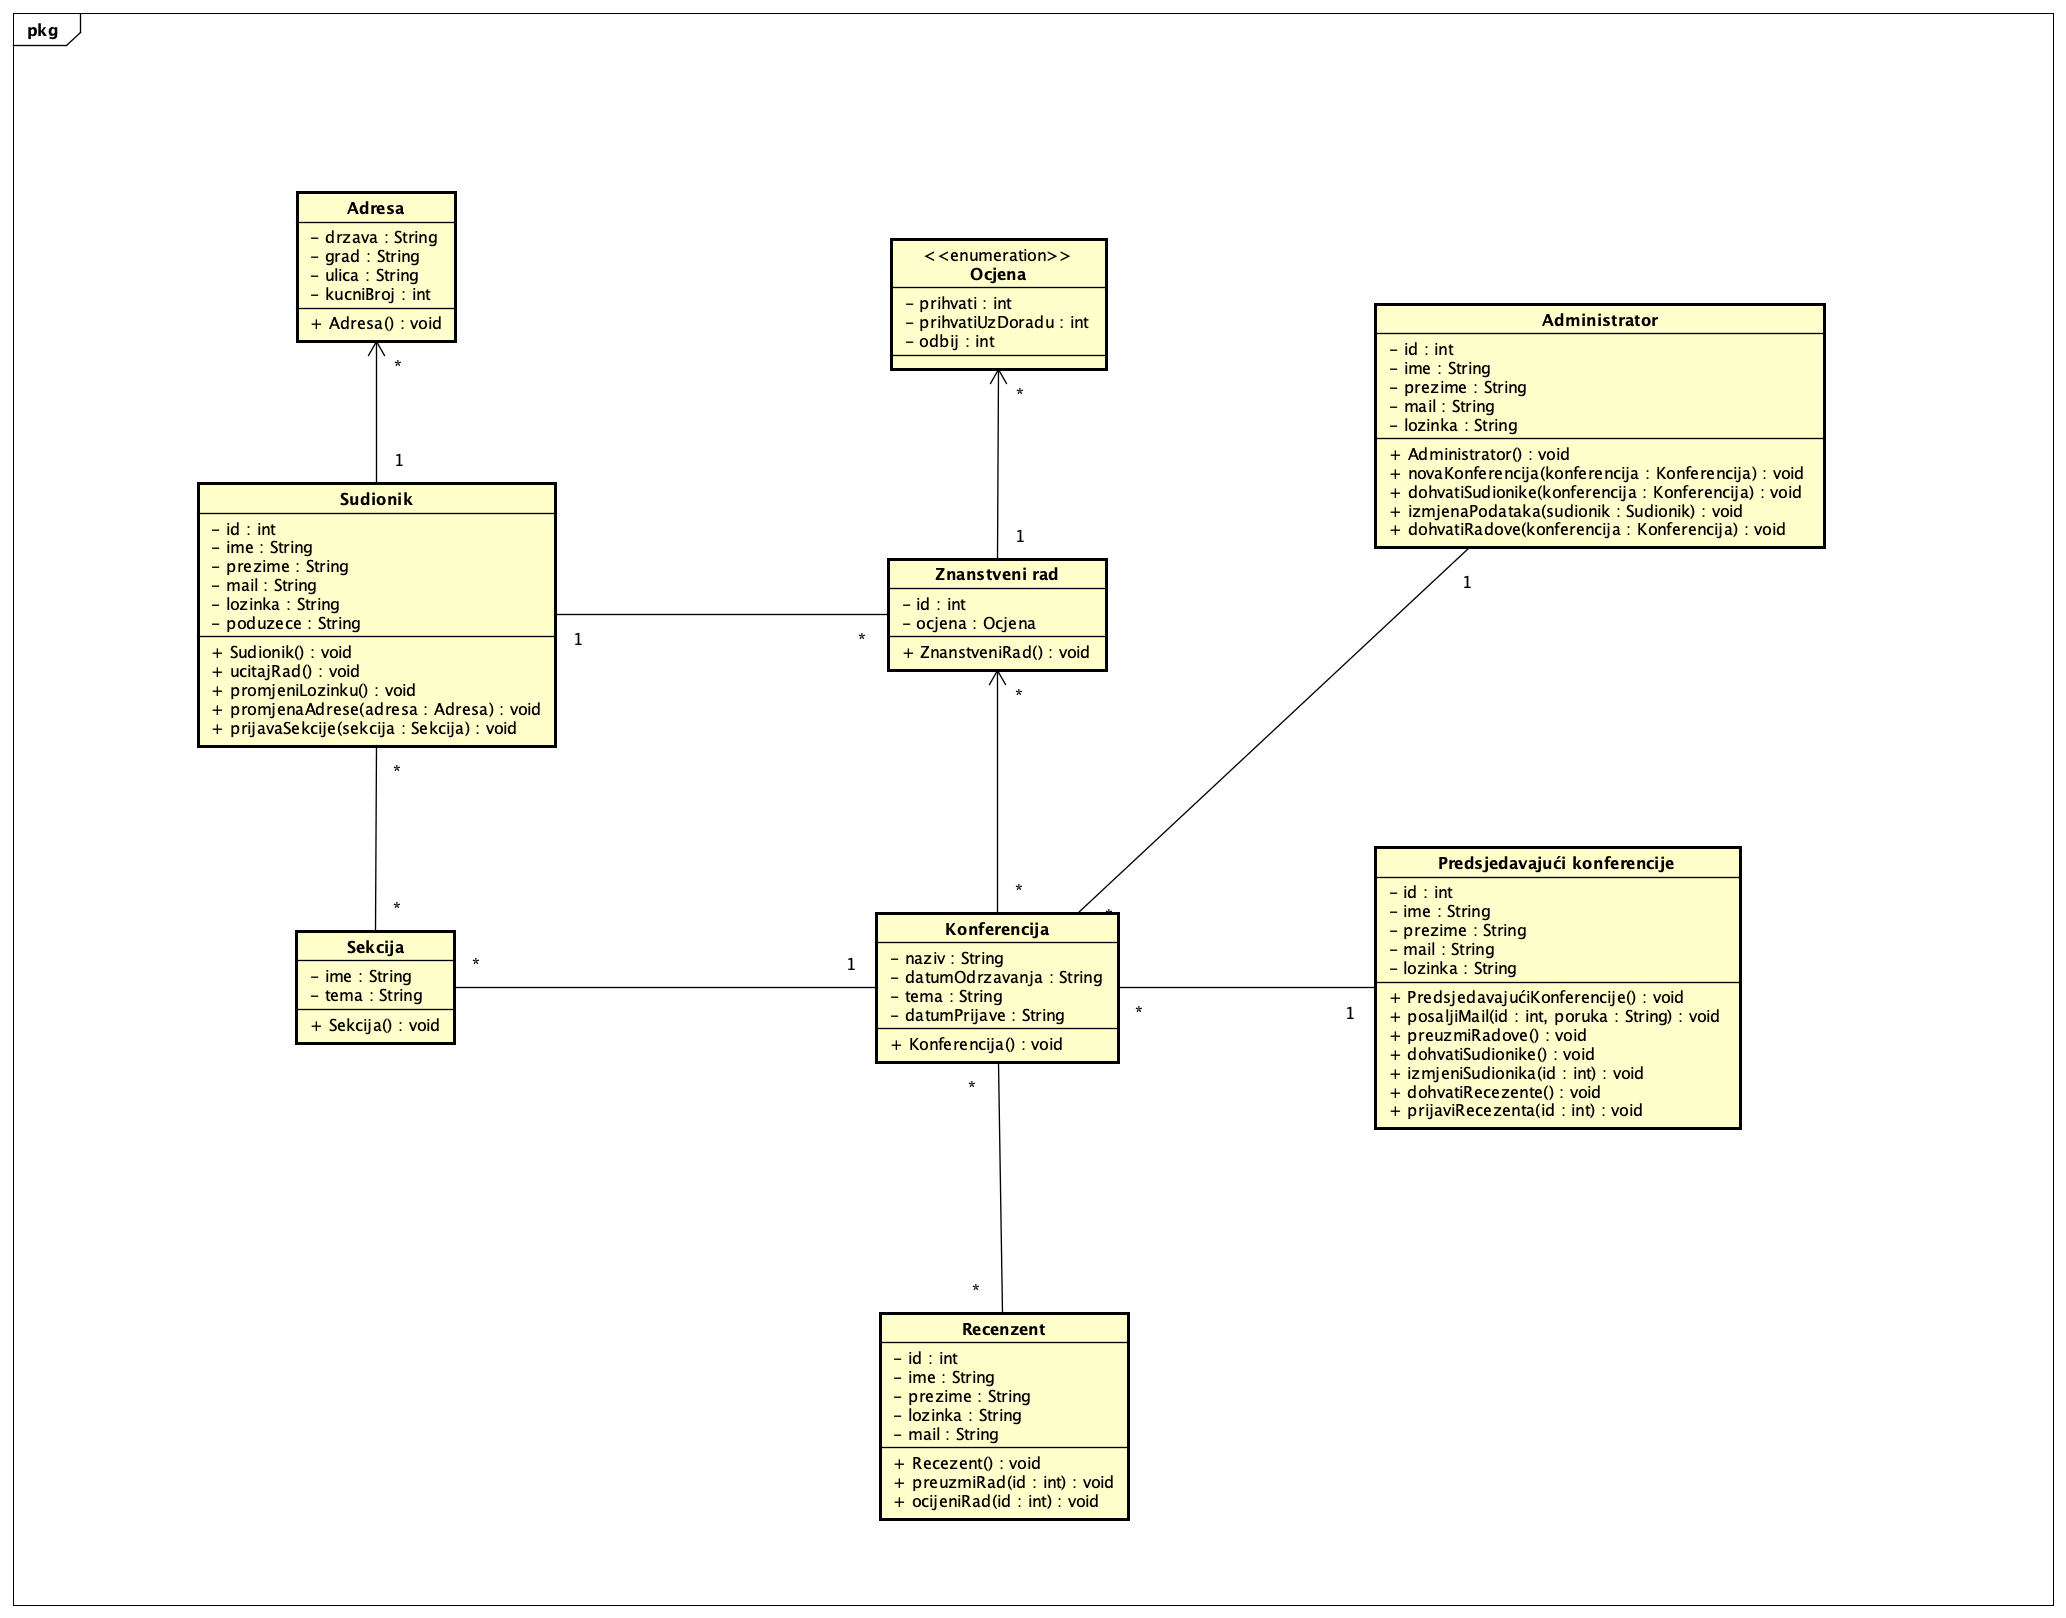
\includegraphics[width=1\linewidth]{slike/ClassDiagramSlika} %veličina u odnosu na širinu linije
				\centering
				\caption{Dijagram razreda}
				\label{Class Diagram} %label mora biti drugaciji za svaku sliku
			\end{figure}
		
			\eject
			
		\section{Dijagram stanja}
			Dijagram stanja prikazuje stanje objekta te prijelaze iz jednog stanja u drugo temeljene na događajima. Na slici 4.3 prikazan je dijagram stanja za Korisnika. Nakon uspješne prijave korisniku se prikazuje početna stranica na kojoj može odabrati više opcija. Klikom na Popis konferencija mu se prikazuju konferencije na koje se dalje može prijaviti, a u prijavi odabrati sekciju, unijeti podatke i naposlijetku potvrditi prijavu. Klikom na Učitavanje rada, uz uvjet da mu je odobrena prijava u sekciju te da nije isteklo vrijeme za učitavanje rada, može učitati rad te ga onda poslati. Klikom na Postavke, korisnik može urediti vlastite podatke pa onda izmijenjene podatke spremiti. Također, korisnik u Postavkama može i izbrisati svoj korisnički račun. Klikom na Moji radovi, korisnik može pogledati informacije o svojim radovima, može dohvatiti i urediti učitani rad te onda pohraniti promjene. Korisnik također može klikom na Prijava za recenziranje ispuniti obrazac prijave za recenziranje te ispunjeni obrazac potvrditi i poslati na odobrenje.
			
			\begin{figure}[H]
				\includegraphics[width=1\linewidth]{slike/"Dijagram stanja"} %veličina u odnosu na širinu linije
				\centering
				\caption{Dijagram stanja}
				\label{State Diagram - Korisnik} %label mora biti drugaciji za svaku sliku
			\end{figure}
			
			\eject
		
		\section{Dijagram aktivnosti}
			Dijagram aktivnosti primjenjuje se za opis modela toka upravljanja ili toka podataka. Ne upotrebljava se za modeliranje događajima poticanog ponašanja. U modeliranju toka upravljanja svaki novi korak poduzima se nakon završenog prethodnog, a naglasak je na jednostavnosti. Na dijagramu 4.4 prikazan je proces prijave za sudjelovanje na konferenciji. Korisnik unese podatke za prijavu u sustav, odabere popis konferencija te odabere konferenciju i sekciju u njoj. Naposljetku, korisnik unese podatke za prijavu te ga aplikacija vrati na početnu stranicu.
			
			\begin{figure}[H]
				\includegraphics[width=1\linewidth]{slike/"Dijagram aktivnosti"} %veličina u odnosu na širinu linije
				\centering
				\caption{Dijagram aktivnosti}
				\label{Activity Diagram - Prijava za sudjelovanje na konferenciji} %label mora biti drugaciji za svaku sliku
			\end{figure}
			
			\eject
			
		\section{Dijagram komponenti}
			Dijagram komponenti na slici 4.5 opisuje organizaciju i međuovisnost komponenti, interne strukture i odnose prema okolini. Preko sučelja za dohvat datoteka i JSON-a pristupa se app.js komponenti. Frontend se sastoji od HTML datoteka koje se nalaze u direktoriju "views", dok je Javascript kod backenda koji je zadužen za upravljanje rutama u diretkriju "routes".
			Postgres je zadužen za dohvaćanje tablica iz baze podataka pomoću SQL upita. Podaci koji su pristigli dalje se šalju u queries.js.
			
			\begin{figure}[H]
				\includegraphics[width=1\linewidth]{slike/"Dijagram komponenti"} %veličina u odnosu na širinu linije
				\centering
				\caption{Dijagram komponenti}
				\label{Component Diagram} %label mora biti drugaciji za svaku sliku
			\end{figure}		
 	\chapter{Implementacija i korisničko sučelje}
		
		
		\section{Korištene tehnologije i alati}
			Komunikacija u timu realizirana je korištenjem aplikacija Whatsapp i Discord. Za izradu UML dijagrama korišten je alat Astah Professional, a kao sustav za upravljanje izvornim kodom Git. Udaljeni repozitorij projekta je dostupan na web platformi GitLab.\par
			
			Kao razvojno okruženje korišten je Visual Studio Code - integrirano razvojno okruženje (IDE) tvrtke Microsoft.\par
			
			Udaljeni repozitorij projekta je dostupan na web platformi GitLab.\par
			
			Aplikacija je napisana koristeći Node.js-a za izradu \textit{backenda} te Embedded Javascript za izradu \textit{frontenda}.\par 
			
			Baza podataka je izrađena u PostgreSQL-u.\par
			
			
			\eject 
		
	
		\section{Ispitivanje programskog rješenja}
			
			\subsection{Ispitivanje komponenti}
			\textit{Potrebno je provesti ispitivanje jedinica (engl. unit testing) nad razredima koji implementiraju temeljne funkcionalnosti. Razraditi \textbf{minimalno 6 ispitnih slučajeva} u kojima će se ispitati redovni slučajevi, rubni uvjeti te izazivanje pogreške (engl. exception throwing). Poželjno je stvoriti i ispitni slučaj koji koristi funkcionalnosti koje nisu implementirane. Potrebno je priložiti izvorni kôd svih ispitnih slučajeva te prikaz rezultata izvođenja ispita u razvojnom okruženju (prolaz/pad ispita). }
			
			
			
			\subsection{Ispitivanje sustava}
			
			 Testirali smo dva segmenta aplikacije: registraciju korisnika i prijavu korisnika
			 		
			 	\subsubsection{Registracija korisnika}	
			 		\textbf{Slučaj 1}\\
			 		Opis ispitnog slučaja:
			 		\begin{itemize}
			 			\item Radimo registraciju korisnika. Svi ulazni podaci su ispravni osim unesene e-mail adrese koja je već korištena za prijavu jednog od korisnika
			 		\end{itemize}
		 			Očekivani rezultat:
		 			\begin{itemize}
		 				\setlength\itemsep{0.1em}
		 				\item Neuspješna registracija
		 				\item Ispis "E-mail koji ste odabrali se već koristi."
		 			\end{itemize}
	 				\begin{figure}[H]
	 					\includegraphics[width=0.8\linewidth]{slike/"registracija korisnika FAIL - selenium"}
	 					\centering
	 					\caption{Registracija korisnika FAIL - selenium}
	 					\label{registracija korisnika FAIL - selenium}
	 				\end{figure}
 					Dobiveni rezultat:
 					\begin{itemize}
 						\setlength\itemsep{0.1em}
 						\item Neuspješna prijava
 						\item Ispis primjerene poruke
 					\end{itemize}
 					\begin{figure}[H]
 						\includegraphics[width=0.5\linewidth]{slike/"neuspjesna registracija"}
 						\centering
 						\caption{Neuspješna registracija - e-mail se već koristi}
 						\label{neuspjesna registracija - e-mail se vec koristi}
 					\end{figure}
 					
 					\textbf{Slučaj 2}\\
 					Opis ispitnog slučaja:
 					\begin{itemize}
 						\item Radimo registraciju korisnika. Svi podaci su ispravno uneseni
 					\end{itemize}
 					Očekivani rezultat:
 					\begin{itemize}
 						\setlength\itemsep{0.1em}
 						\item Uspješna registracija
 						\item Ispis "Na vašu e-mail adresu dostavljena je lozinka i aktivacijski link. Molimo prvo potvrdite svoju registraciju."
 					\end{itemize}
 					\begin{figure}[H]
 						\includegraphics[width=1\linewidth]{slike/"registracija korisnika OK - selenium"}
 						\centering
 						\caption{Registracija korisnika OK - selenium}
 						\label{registracija korisnika OK - selenium}
 					\end{figure}
 					Dobiveni rezultat:
 					\begin{itemize}
 						\setlength\itemsep{0.1em}
 						\item Uspješna registracija
 						\item Ispis poruke
 					\end{itemize}
 					\begin{figure}[H]
 						\includegraphics[width=0.5\linewidth]{slike/"uspjesna registracija"}
 						\centering
 						\caption{Uspješna registracija - poruka}
 						\label{uspjesna registracija}
 					\end{figure}
		 		\eject
		 		
		 		\subsubsection{Prijava korisnika}
		 			\textbf{Slučaj 1}\\
		 			Opis ispitnog slučaja:
		 			\begin{itemize}
		 				\item Korisnik se prijavljuje u sustav
		 			\end{itemize}
	 				Očekivani rezultat:
	 				\begin{itemize}
	 					\item Uspješna prijava u sustav
	 				\end{itemize}
 					\begin{figure}[H]
 						\includegraphics[width=1\linewidth]{slike/"prijavaKorisnika_OK-selenium"}
 						\centering
 						\caption{Prijava korisnika OK -selenium}
 						\label{uspjesna prijava - selenium}
 					\end{figure}
 					Dobiveni rezultat:
 					\begin{itemize}
 						\item Korisnik se uspješno prijavio u sustav
 					\end{itemize}
 					\begin{figure}[H]
 						\includegraphics[width=0.9\linewidth]{slike/"uspjesnaPrijava-prikazProfila"}
 						\centering
 						\caption{Uspješna prijava}
 						\label{uspjesna prijava}
 					\end{figure}
 				
 					\textbf{Slučaj 2}\\
 					Opis ispitnog slučaja:
 					\begin{itemize}
 						\item Pokušaj prijave korisnika u sustav s nepotvrđenim računom
 					\end{itemize}
 					Očekivani rezultati:
 					\begin{itemize}
 						\setlength\itemsep{0.1em}
 						\item Neuspješna prijava
 						\item Ispis "Vaša registracija nije potvrđena. Potvrdite e-mail"
 					\end{itemize}
 					\begin{figure}[H]
 						\includegraphics[width=1\linewidth]{slike/"prijavaKorisnika_FAIL-selenium"}
 						\centering
 						\caption{Prijava korisnika FAIL - selenium}
 						\label{neuspjesna prijava - selenium}
 					\end{figure}
 					Dobiveni rezultati:
 					\begin{itemize}
 						\setlength\itemsep{0.1em}
 						\item Neuspješna prijava
 						\item prikaz poruke
 					\end{itemize}
 					\begin{figure}[H]
 						\includegraphics[width=0.5\linewidth]{slike/"neuspjesnaPrijava"}
 						\centering
 						\caption{Neuspješna prijava - nepotvrđena registracija}
 						\label{neuspjesna prijava}
 					\end{figure}
			
			\eject 
			
			
			\textbf{Slučaj 2}\\
			Opis ispitnog slučaja:
			\begin{itemize}
				\item Pokušaj prijave korisnika u sustav s nepotvrđenim računom
			\end{itemize}
			Očekivani rezultati:
			\begin{itemize}
				\setlength\itemsep{0.1em}
				\item Neuspješna prijava
				\item Ispis "Vaša registracija nije potvrđena. Potvrdite e-mail"
			\end{itemize}
			\begin{figure}[H]
				\includegraphics[width=1\linewidth]{slike/"prijavaKorisnika_FAIL-selenium"}
				\centering
				\caption{Prijava korisnika FAIL - selenium}
				\label{neuspjesna prijava - selenium}
			\end{figure}
			Dobiveni rezultati:
			\begin{itemize}
				\setlength\itemsep{0.1em}
				\item Neuspješna prijava
				\item prikaz poruke
			\end{itemize}
			\begin{figure}[H]
				\includegraphics[width=0.5\linewidth]{slike/"neuspjesnaPrijava"}
				\centering
				\caption{Neuspješna prijava - nepotvrđena registracija}
				\label{neuspjesna prijava}
			\end{figure}
			
			\eject 
			
			
			\subsubsection{Stvaranje konferencije}
			\textbf{Slučaj 1}\\
			Opis ispitnog slučaja:
			\begin{itemize}
				\item Administrator stvara novu konferenciju
			\end{itemize}
			Očekivani rezultat:
			\begin{itemize}
				\item Konferencija uspješno stvorena
			\end{itemize}
			\begin{itemize}
				\item Ispis odgovarajuće poruke
			\end{itemize}
			\begin{figure}[H]
				\includegraphics[width=1\linewidth]{slike/"selenium - stvaranje konf"}
				\centering
				\caption{Stvaranje konferencije OK - selenium}
				\label{uspjesna prijava - selenium}
			\end{figure}
			Dobiveni rezultat:
			\begin{itemize}
				\item Konferencija uspješno stvorena
			\end{itemize}
			\begin{itemize}
				\item Ispis poruke o uspjehu
			\end{itemize}
			\begin{figure}[H]
				\includegraphics[width=0.9\linewidth]{slike/"stvaranje konf - uspjeh"}
				\centering
				\caption{Uspješna prijava}
				\label{uspjesna prijava}
			\end{figure}
		
		\subsubsection{Prijava za sudjelovanje na konferenciji}
		\textbf{Slučaj 1}\\
		Opis ispitnog slučaja:
		\begin{itemize}
			\item Korisnik među ponuđenim konferencijama odabire onu na kojoj želi sudjelovati. Preduvjet je da je do trenutka odabira željene konferencije barem jedna konferencija definirana (uključujući njenog organizatora i sekcije). Klikom na gumb 'Prijava za sudjelovanje' korisniku se otvara forma koju treba ispuniti, a koja uključuje popis imena svih sekcija odabrane konferencije i prostor za upis vlastitog imena i prezimena. Nakon popunjavanja navedenih podataka klikom na gumb prijava se šalje u sustav.
		\end{itemize}
		Očekivani rezultat:
		\begin{itemize}
			\item Prijava je uspješno zabilježena u sustavu i korisnik prima elektroničkom poštom potvrdu u kojoj su zabilježeni njegovi osobni podatci uz podatke koji opisuju odabranu konferenciju i rok pohranjivanja znanstvenog rada u sustav.
		\end{itemize}
		\begin{itemize}
			\item Ispis poruke koja potvrđuje uspješnu prijavu u okviru koji odgovara konferenciji koja ja prethodno odabrana.
		\end{itemize}
		\begin{figure}[H]
			\includegraphics[width=1\linewidth]{slike/"marko_test_1"}
			\centering
			\caption{Uspješna potvrda prijave - selenium}
			\label{mala_labelica}
		\end{figure}
		Dobiveni rezultat:
		\begin{itemize}
			\item Prijava uspješno zabilježena u sustav
		\end{itemize}
		\begin{itemize}
			\item Ispis poruke o uspjehu
		\end{itemize}
		\begin{figure}[H]
			\includegraphics[width=0.9\linewidth]{slike/"marko_screen_1"}
			\centering
			\caption{Uspješna prijava}
			\label{mala_labelica}
		\end{figure}
		
		
		\section{Dijagram razmještaja}
			Dijagrami razmještaja opisuju topologiju sklopovlja i programsku potporu koja se koristi u implementaciji sustava u njegovom radnom okruženju.Na poslužiteljskom	računalu se nalaze web poslužitelj i poslužitelj baze podataka. Klijenti koriste web preglednik kako bi pristupili web aplikaciji. Sustav je baziran na arhitekturi ”klijent – poslužitelj”, a komunikacija između računala korisnika i poslužitelja odvija se preko HTTP veze.\\
			\begin{figure}[H]
				\includegraphics[width=1\linewidth]{slike/"Dijagram razmjestaja"}
				\centering
				\caption{Dijagram razmještaja}
				\label{dijagram razmjestaja}
			\end{figure}
						
			\eject 
		
		\section{Upute za puštanje u pogon}
		
			
			 
			
			\definecolor{light-gray}{gray}{0.95}
			\newcommand{\code}[1]{\colorbox{light-gray}{\texttt{#1}}}
			 
			 Web servis se može pustiti u pogon na bilo kojem poslužitelju. U ovoj uputi će se koristiti poslužitelj \textit{Heroku} s besplatnim planom.
			 
			 Posjetite \href{https://www.heroku.com/}{Heroku web stranicu} te napravite besplatni račun. Zatim potvrdite svoj račun i odaberite plan svog računa \href{https://devcenter.heroku.com/articles/account-verification}{ovdje}. Zatim instalirajte i dodajte u lokalnu varijablu \textit{PATH} Heroku CLI pomoću web stranice \href{https://devcenter.heroku.com/articles/getting-started-with-nodejs#set-up}{ovdje}. Nakon toga otvorite naredbeni redak u praznoj mapi gdje će te klonirati javni repozitorij. Izvršite naredbu:
			 
			 \code{git clone https://gitlab.com/andreism/grupa1.git}
			 
			 \noindent
			 Zatim se pozicionirajte u novonastalu mapu pomoću:
			 
			 \code{cd grupa1}
			 
			 \noindent
			 Zatim izvršite naredbu:
			 
			 \code{heroku create svoje-ime}
			 
			 \noindent
			 umjesto "svoje-ime" stavite proizvoljno ime. Dalje izvršite naredbu:
			 
			 \code{git push heroku master}
			 
			 \noindent
			 kako biste postavili server na poslužitelja. Još je preostalo podešavanje baze podataka. Za to posjetite svoj \href{https://dashboard.heroku.com/apps}{\textit{Heroku dashboard}} te kliknite na svoju aplikaciju koju ste prethodno napravili. Zatim kliknite na gumb \textit{More} 
			 
			 \begin{figure}[H]
			 	\includegraphics[width=0.9\linewidth]{upute-slike/"more"}
			 	\centering
			 	\caption{Tipka \textit{More}}
			 	\label{mala_labelica}
			 \end{figure}
			 
			 te odaberite opciju \textit{Run console}. 
			 
			 \begin{figure}[H]
			 	\includegraphics[width=0.9\linewidth]{upute-slike/"run-console"}
			 	\centering
			 	\caption{Tipka \textit{Run console}}
			 	\label{mala_labelica}
			 \end{figure}
			 
			 Upišite u polje \textit{bash} te kliknite gumb \textit{Run} 
			 
			 \begin{figure}[H]
			 	\includegraphics[width=0.9\linewidth]{upute-slike/"bash-run"}
			 	\centering
			 	\caption{\textit{Bash run}}
			 	\label{mala_labelica}
			 \end{figure}
			 
			 pričekajte dok se ne pojave znakovi
			 \code{\textasciitilde  \$} u konzoli. Kada se pojave znakovi \code{\textasciitilde  \$} u konzoli, izvršite komandu:
			 
			 \code{npm run seed}
			 
			 \noindent
			 te pričekajte da se naredba izvrši do kraja. Nakon što je naredba gotova, možete zatvoriti konzolu. Web servis je sada spreman i dostupan. Web stranicu možete posjetiti pomoću \textit{Open app} gumba
			 
			 \begin{figure}[H]
			 	\includegraphics[width=0.9\linewidth]{upute-slike/"open-app"}
			 	\centering
			 	\caption{tipka \textit{Open app}}
			 	\label{mala_labelica}
			 \end{figure}
			 
			 
			 
			
			
			\eject 
	\chapter{Zaključak i budući rad}
				
		 Zadatak naše grupe bio je razvoj web aplikacije za organiziranje znanstvenih konferencija uz mogućnost prijavljivanja sudionika, učitavanja znanstvenoga rada od strane prijavljenog sudionika, recenziranja učitanih radova od strane recenzenata, pregled radova lokalno i online od strane organizatora konferencije i recenzenata te uz mogućnosti pridijeljenih administratoru.\\
		 Nakon 15 tjedana rada u timu i razvoja, ostvarili smo zadani cilj. Sama provedba projekta bila je gotova kroz dvije faze.\par
		 		 
		 Prva faza projekta uključivala je okupljanje tima za razvoj aplikacije, dodjelu projektnog zadatka i intenzivan rad na dokumentiranju zahtjeva. Kvalitetna provedba prve faze olakšala je daljnji rad na realizaciji aplikacije.
		 Izrađeni su obrasci i dijagrami (obrasci uporabe, sekvencijski dijagrami, model baze podataka i dijagram razreda). Oni su uvelike pomogli podtimovima zaduženim za razvoj \textit{frontenda} i \textit{backenda}. Vizualizacija samih idejnih rješenja pomoću obrazaca i dijagrama je uštedila mnogo vremena u drugom ciklusu u trenutcima kada su članovi tima nailazili na nedoumice oko implementacije rješenja.\par
		 
		 Druga faza projekta je bila nešto kraća, ali i intezivnija po pitanju samostalnog rada svakog člana tima. Na početku druge faze je urađena podjela tima na one koji će raditi na \textit{frontendu}, one koji će raditi na \textit{backendu} i na one koji će raditi na bazi podataka sukladno njihovim vlastitim željama i iskustvu u tehnologijama u kojima se projekt radio. Osim realizacije rješenja, u drugoj fazi je bilo potrebno dokumentirati ostale UML dijagrame i izraditi popratnu dokumentaciju kako bi budući korisnici mogli lakše koristiti ili vršiti preinake na sustavu.\par
			
		 Komunikacija među članovima je bila putem aplikacija Whatsapp i Discord čime je olakšano informiranje članova o napretku projekta. Upravljanje izvornim kodom se vršilo sustavom Git, a repozitorij projekta nalazi se na se na web platformi GitLab.\par
		
		 Sudjelovanje na ovakvom projektu bilo je vrijedno iskustvo svim članovima tima jer smo kroz 15 tjedana iskusili zajednički rad na projektima. Spoznali smo važnost dobre vremenske organiziranosti i koordiniranosti među članovima tima. U slučaju da bi semestar tj. vrijeme za izradu bilo produženo za barem još jedan ciklus tj. 5-6 tjedana, aplikacija bi bila dotjerana do savršenstva.\\
		 Zadovoljni smo postignutim bez obzira na neke teškoće i u komunikaciji i u samom razvoju aplikacije te smatramo da smo ovim projektom dobili iskustvo i barem donekle dočarali što nas čeka nakon završetka školovanja.
		\eject 
	\chapter*{Popis literature}
		\addcontentsline{toc}{chapter}{Popis literature}
	 	
 	
		
		
		\begin{enumerate}
			
			
			\item  Programsko inženjerstvo, FER ZEMRIS, \url{http://www.fer.hr/predmet/proinz}
			
			\item  I. Sommerville, "Software engineering", 8th ed, Addison Wesley, 2007.
			
			\item  T.C.Lethbridge, R.Langaniere, "Object-Oriented Software Engineering", 2nd ed. McGraw-Hill, 2005.
			
			\item  I. Marsic, Software engineering book``, Department of Electrical and Computer Engineering, Rutgers University, \url{http://www.ece.rutgers.edu/~marsic/books/SE}
			
			\item  The Unified Modeling Language, \url{https://www.uml-diagrams.org/}
			
			\item  Astah Community, \url{http://astah.net/editions/uml-new}
		\end{enumerate}
		
		 
	
	
	\begingroup
	\renewcommand*\listfigurename{Indeks slika i dijagrama}
	%\renewcommand*\listtablename{Indeks tablica}
	%\let\clearpage\relax
	\listoffigures
	%\vspace{10mm}
	%\listoftables
	\endgroup
	\addcontentsline{toc}{chapter}{Indeks slika i dijagrama}


	
	\eject 
		
	\chapter*{Dodatak: Prikaz aktivnosti grupe}
		\addcontentsline{toc}{chapter}{Dodatak: Prikaz aktivnosti grupe}
		
		\section*{Dnevnik sastajanja}
		
		\begin{packed_enum}
			\item  sastanak
			
			\item[] \begin{packed_item}
				\item Datum: 6. listopada 2020.
				\item Prisustvovali: M.Andreis, S.Andričević, M.Bašić, T.Krešo, B.Majstorović, T.Matić, P.Pasković, M.Krhen, M.Sušilović 
				\item Teme sastanka:
				\begin{packed_item}
					\item  sastanak s asistentom i demonstratorom
					\item  raščišćavanje osnovnih dilema funkcionalnosti
					\item analiza zadatka
				\end{packed_item}
			\end{packed_item}
			
			\item  sastanak
			\item[] \begin{packed_item}
				\item Datum: 17. listopada 2020.
				\item Prisustvovali: M.Andreis, S.Andričević, M.Bašić, T.Krešo, B.Majstorović, T.Matić, P.Pasković
				\item Teme sastanka:
				\begin{packed_item}
					\item  definiranje funkcionalnih zahtjeva
					\item  podjela opisa obrazaca uporabe
				\end{packed_item}
			\end{packed_item}
		
		\item  sastanak
		\item[] \begin{packed_item}
			\item Datum: 20. listopada 2020.
			\item Prisustvovali: M.Andreis, S.Andričević, M.Bašić, T.Krešo, B.Majstorović, T.Matić, P.Pasković, M.Krhen, M.Sušilović
			\item Teme sastanka:
			\begin{packed_item}
				\item  sastanak s asistentom i demosom - prodiskutirati dosadašnji rad (fokus na opisima obrazaca uporabe)
				\item  podijeliti dalje poslove
			\end{packed_item}
		\end{packed_item}
	
		\item  sastanak
		\item[] \begin{packed_item}
			\item Datum: 25. listopada 2020.
			\item Prisustvovali: M.Andreis, S.Andričević, M.Bašić, T.Krešo, B.Majstorović, T.Matić, P.Pasković
			\item Teme sastanka:
			\begin{packed_item}
				\item  podjela zadataka (sekvencijski dijagrami + dodani obrasci + popravak dijagrama obrazaca uporabe)
			\end{packed_item}
		\end{packed_item}
	
	\item  sastanak
	\item[] \begin{packed_item}
		\item Datum: 27. listopada 2020.
		\item Prisustvovali: M.Andreis, S.Andričević, M.Bašić, T.Krešo, B.Majstorović, T.Matić, P.Pasković, M.Krhen, M.Sušilović
		\item Teme sastanka:
		\begin{packed_item}
			\item  sastanak s asistentom - komentiranje dijagrama obrazaca i sekvencijskih dijagrama
			\item daljnja podjela rada
		\end{packed_item}
	\end{packed_item}

	\item  sastanak
	\item[] \begin{packed_item}
		\item Datum: 3. studenog 2020.
		\item Prisustvovali: M.Andreis, S.Andričević, M.Bašić, T.Krešo, B.Majstorović, T.Matić, P.Pasković
		\item Teme sastanka:
		\begin{packed_item}
			\item osmišljavanje stranice i pojedinih pregleda
			\item  dogovor za rad oko implementacije generičkih funkcionalnosti aplikacije
		\end{packed_item}
	\end{packed_item}

\item  sastanak
\item[] \begin{packed_item}
	\item Datum: 3. studenog 2020.
	\item Prisustvovali: M.Andreis, S.Andričević, M.Bašić, T.Krešo, B.Majstorović, T.Matić, P.Pasković, M.Krhen, M.Sušilović
	\item Teme sastanka:
	\begin{packed_item}
		\item sastanak s asistentom - demonstracije generičkih funkcionalnosti aplikacije
		\item daljnja podjela rada
	\end{packed_item}
\end{packed_item}

\item  sastanak
\item[] \begin{packed_item}
	\item Datum: 4. prosinca 2020.
	\item Prisustvovali: M.Andreis, S.Andričević, M.Bašić, T.Krešo, B.Majstorović, T.Matić, P.Pasković
	\item Teme sastanka:
	\begin{packed_item}
		\item komentiranje dotad učinjenog
		\item daljnja podjela rada
	\end{packed_item}
\end{packed_item}

\item  sastanak
\item[] \begin{packed_item}
	\item Datum: 16. prosinca 2020.
	\item Prisustvovali: M.Andreis, S.Andričević, M.Bašić, T.Krešo, B.Majstorović, T.Matić, P.Pasković
	\item Teme sastanka:
	\begin{packed_item}
		\item komentiranje dotad učinjenog
		\item dogovor o poboljšanju nekih stavki
		\item daljnja podjela rada
	\end{packed_item}
\end{packed_item}

\item  sastanak
\item[] \begin{packed_item}
	\item Datum: 21. prosinca 2020.
	\item Prisustvovali: M.Andreis, S.Andričević, M.Bašić, T.Krešo, B.Majstorović, T.Matić, P.Pasković
	\item Teme sastanka:
	\begin{packed_item}
		\item dogovor za početak izrade 2. dijela dokumentacije
		\item daljnja podjela rada
	\end{packed_item}
\end{packed_item}

\item  sastanak
\item[] \begin{packed_item}
	\item Datum: 8. siječnja 2021.
	\item Prisustvovali: M.Andreis, S.Andričević, M.Bašić, T.Krešo, B.Majstorović, T.Matić, P.Pasković, M.Krhen, M.Sušilović
	\item Teme sastanka:
	\begin{packed_item}
		\item sastanak s asistentom - prezentiranje alfa verzije aplikacije
		\item dogovor za dovršavanje dokumentacije
		\item daljnja podjela rada
	\end{packed_item}
\end{packed_item}

			
			%
			
		\end{packed_enum}
		
		\eject
		\section*{Tablica aktivnosti}
					
			
			\begin{longtabu} to \textwidth {|X[7, l]|X[1, c]|X[1, c]|X[1, c]|X[1, c]|X[1, c]|X[1, c]|X[1, c]|}
								
				\cline{2-8} \multicolumn{1}{c|}{\textbf{}} &     \multicolumn{1}{c|}{\rotatebox{90}{\textbf{Marko Andreis }}} & \multicolumn{1}{c|}{\rotatebox{90}{\textbf{Stjepan Andričević }}} &	\multicolumn{1}{c|}{\rotatebox{90}{\textbf{Mario Bašić }}} &	\multicolumn{1}{c|}{\rotatebox{90}{\textbf{Toni Krešo }}} &
				\multicolumn{1}{c|}{\rotatebox{90}{\textbf{Borna Majstorović }}} &
				\multicolumn{1}{c|}{\rotatebox{90}{\textbf{Toni Matić }}} &	\multicolumn{1}{c|}{\rotatebox{90}{\textbf{Pero Pasković }}} \\ \hline 
				\endfirsthead
				
			
				\cline{2-8} \multicolumn{1}{c|}{\textbf{}} &     \multicolumn{1}{c|}{\rotatebox{90}{\textbf{Marko Andreis }}} & \multicolumn{1}{c|}{\rotatebox{90}{\textbf{Stjepan Andričević }}} &	\multicolumn{1}{c|}{\rotatebox{90}{\textbf{Mario Bašić }}} &
				\multicolumn{1}{c|}{\rotatebox{90}{\textbf{Toni Krešo }}} &	\multicolumn{1}{c|}{\rotatebox{90}{\textbf{Borna Majstorović }}} &
				\multicolumn{1}{c|}{\rotatebox{90}{\textbf{Toni Matić }}} &	\multicolumn{1}{c|}{\rotatebox{90}{\textbf{Pero Pasković }}} \\ \hline 
				\endhead
				
				
				\endfoot
							
				 
				\endlastfoot
				
				Upravljanje projektom 		& 4 &  & 2 &  &  & 2 &  \\ \hline
				Opis projektnog zadatka 	& 2 & 1 & 2 &  &  & 2 & 1 \\ \hline
				
				Funkcionalni zahtjevi       & 2 & 1 & 2 & 2 & 3 & 2 &  \\ \hline
				Opis pojedinih obrazaca 	& 4 & 2 & 3 & 1 & 2 & 4 & 1 \\ \hline
				Dijagram obrazaca 			& 3 &  & 5 & 1 & 1 & 3 & 1 \\ \hline
				Sekvencijski dijagrami 		&  & 5 &  & 1 &  & 1 & 4 \\ \hline
				Opis ostalih zahtjeva 		& 1 & 1 & 1 & 2 & 1 & 2 & 1 \\ \hline

				Arhitektura i dizajn sustava	 & 3 & 2 & 2 & 3 &  & 3  & 2 \\ \hline
				Baza podataka				&  & 1 & 1 & 5 &  & 1 & 1  \\ \hline
				Dijagram razreda 			& 1 & 3 & 1 & 2 & 5 & 1 & 1  \\ \hline
				Dijagram stanja				&  & 4 &  &  &  & 4 & 2 \\ \hline
				Dijagram aktivnosti 		&  & 4 &  &  &  & 4 & 2 \\ \hline
				Dijagram komponenti			&  & 4 &  &  &  & 4 & 2 \\ \hline
				Korištene tehnologije i alati 		&  &  & 1 & 1 &  &  & 4 \\ \hline
				Ispitivanje programskog rješenja 	&  & 4 &  &  &  & 4 &  \\ \hline
				Dijagram razmještaja			&  & 4 &  &  &  & 4 & 2 \\ \hline
				Upute za puštanje u pogon 		&  & 4 &  &  &  & 4 &  \\ \hline 
				Dnevnik sastajanja 			& 1 & 1 & 1 & 1 & 1 & 1 &  \\ \hline
				Zaključak i budući rad 		& 1 &  & 1 &  &  &  & 5 \\  \hline
				Popis literature 			&  & 1 &  &  & 2 &  & 1 \\  \hline
				&  &  &  &  &  &  &  \\ \hline \hline
				
				
				\textit{izrada početne stranice} 				&  &  &  &  & 1 & 3 &  \\ \hline 
				\textit{izrada baze podataka} 		 			&  &  &  & 5 & 1 &  & \\ \hline 
				\textit{spajanje s bazom podataka} 							& 1 &  &  &  &  &  &  \\ \hline
				\textit{back end} 							& 1 & 3 & 4 &  & 4 &  &  \\  \hline
				 						
				
				
			\end{longtabu}

	


\end{document} %naredbe i tekst nakon ove naredbe ne ulaze u izgrađen dokument 


